\chapter[A Lighthouse in the Dust]{A Lighthouse in the Dust: Reverberation of Periodic Emission from Massive Black Hole Binaries}
\label{ch:Dust}
\let\thefootnote\relax\footnotetext{We dedicate this work to the memory of Arlin Crotts who passed away on November 19, 2015. As an expert on supernovae light echoes, we sorely missed his collaboration on this work.}





\section{Introduction} 

Massive black holes (MBHs) exist at the centers of most, if not all, galaxies
\citep{kr95, KormendyHo2013}. Galactic mergers can deliver MBHs, as well as an
ample supply of gas \citep{BH1992, Barnes:1996, Barnes:2002,
Mayer:2013:MBHBGasRev}, to the centers of newly coalesced galaxies where the
MBHs form a binary. The interaction of massive black hole binaries (MBHBs)
with gas and surrounding stars can drive the pair to sub-pc separations where
gravitational radiation reaction drives the binary to coalescence
\citep{Begel:Blan:Rees:1980}.  Characterization of the population of such sub-pc 
binaries, through present electromagnetic (EM), and future gravitational
wave (GW) channels will provide a powerful tool for understanding the mutual
build-up of galaxies and their central black holes
\citep[\textit{e.g.}][]{KormendyHo2013}, the dynamics of gas and stars in
galactic nuclei \citep[\textit{e.g.}][]{MerrittMilos:2005:LRR}, and the low-frequency 
gravitational wave background \citep[\textit{e.g.}][]{KocsisSesana:2011, Shannon:2015,
Arzoumanian:2015:SGWB}.

Electromagnetic signatures of MBHBs can arise from their interaction with gas.
Hydrodynamical simulations of gas discs surrounding close MBHBs show that
accretion rates onto a binary can rival, and even exceed the accretion rates
onto a single black hole of an equivalent mass \citep{ShiKrolik:2012,
DHM:2013:MNRAS, Farris:2014, ShiKrolik:2015, MunozLai:2016}. Binary accretion
rates can also be uniquely identifiable. Depending on the ratio of BH masses,
$q \equiv M_2/M_1$ ($M_1>M_2$), the accretion induced emission can be
periodically modulated \citep{Farris:2015:Cool}. For systems with $q \gsim
0.05$, the accretion rate is modulated by the strong perturbations from the
time-dependent binary potential \citep{D'Orazio:CBDTrans:2016}. Periodicity in
the accretion rate, and the resulting luminosity of emission, occur at the
binary orbital period and also twice this period for $0.05 \lsim q \lsim 0.3$.
while for $0.3 \lsim q < 1.0$, an additional periodicity appears at $\sim3
\rightarrow 8\times$ the binary orbital period \citep{ShiKrolik:2012,
DHM:2013:MNRAS, Farris:2014, ShiKrolik:2015, MunozLai:2016}.

In addition to luminosity variations that track accretion rate variability,
luminosity variations occur due to special relativity alone. For binary
components moving at relativistic speeds (greater than a few $\%$ the speed of
light), emission varies in brightness at the period of the binary orbit due to
Doppler boosting \citep{PG1302MNRAS:2015a, PG1302Nature:2015b}.\footnote{For
equal mass binaries on circular orbits, each BH emits at the same rest-frame
luminosity and moves at the same orbital speed but in opposite directions,
hence Doppler-boosting effects are nullified unless one BH can accrete at a
higher rate than the other; such a scenario may occur for eccentric binaries
\citep{MunozLai:2016}.}  For binaries with disparate mass ratios, $q \lsim
0.05$, accretion is steady and dominated by the smaller, secondary BH
\citep{DHM:2013:MNRAS, Farris:2014}. In this case, Doppler boosting is
expected to be the dominant, if not only, source of variability. Even near-
equal mass binaries, for which high amplitude accretion variability is
expected, may emit steadily in their rest frame: if viscous and tidal forcing
timescales which transport matter from the edges of the mini-discs around each
BH down to the BH inner most stable circular orbit are long compared to
accretion rate changes at the mini-disc edges, then luminosity variations may
be muted by buffering in the mini-discs. In this case too, Doppler boosting is
the dominate source of variability from accreting MBHBs.



The Doppler-boosting scenario for periodic emission from MBHBs has recently
been developed to interpret the MBHB candidate PG 1302-102
\citep{Graham+2015a}, which exhibits a nearly sinusoidal periodicity in the
V-band continuum. Given the measured binary mass, period, and spectral slope
of PG 1302, \cite{PG1302Nature:2015b} showed that the observed amplitude of
variability in the V-band and ultra-violet (UV) wavelengths is consistent with
that expected for Doppler boosting of emission from an accretion disc around
the secondary BH. Further confirmation of the Doppler-boosting model for PG
1302 requires continued, long-term observations of the system in optical and
UV wavelengths. However measurements in other wavelengths can provide
additional clues to the nature of the central engine of PG 1302.

Such clues have recently come from the infrared (IR). \cite{Jun:2015}
(hereafter J15) analyze data from the WISE satellite to report a periodicity
in the IR continuum of PG 1302 which is consistent with the optical period,
but with a diminished amplitude and at a phase lag of $335 \pm 153$ days in
the W1 band and $524 \pm 148$ days in the W2 band. J15 attribute this phase
lag to reprocessing of the UV/optical continuum of PG 1302 by a surrounding
dust torus at $\sim$pc distances from the illuminating source.

In this work we develop a toy model to interpret the findings of J15 and, in
general, reverberated IR emission from MBHBs. We considers heating of nuclear
dust by periodically varying emission from a central source. We consider a
central source exhibiting spatially isotropic emission and compare to a source
exhibiting anisotropic, Doppler-boosted emission, illuminating the dust
structure as it sweeps around like a lighthouse at the binary orbital
frequency. We crucially take into account the relative light travel time to
different parts of the dust structure in a smooth dust-torus model, centered
on the emitting source, which is optically thick to UV/optical and optically
thin to IR dust emission. We find that the relative magnitude and phase lag of
the reverberated IR emission is dependent not only on the size of the dust
region, but also on its geometry and the pattern speed of the variable
illuminating source. We identify the ratio of source variability period to
light travel time from source to dust as a key parameter setting the amplitude
and phase of the reverberated periodic IR light curve. The phase lag of IR
light curves in the case of a Doppler-boosted source is one quarter cycle
different than the analogous case for an isotropic source. We find also that,
for Doppler boosted emission models, depending on the relative inclination
angles of the binary and the dust torus to the observer's line of sight,
variability can be present in both optical and IR, or in one band and not the
other. This means that present optical surveys of MBHB candidates may have
missed some candidates, with Doppler-boost sources of variability, that vary
only in the reverberated IR. This result motivates an IR plus optical search
for periodic quasars.


% As an example of the utility of our models for dust reverberation of a
% periodic source, We apply them to interpret the IR emission from MBHB
% candidate PG 1302. 
% We find two possible scenarios consistent with the IR light
% curves from WISE. In corroboration with previous analyses of the UV and
% optical data, the IR data for PG 1302 suggests that the periodic IR emission
% is consistent with reverberated emission by the inner edge of a dust disc (or ring),
% with aspect ratio $\pm0.13 \pm 0.06$, in two possible scenarios:
% \begin{enumerate}
% \item An isotropic source surrounded by a nearly \textit{face-on disc} 
% with inner radius $4.1 \pm 0.7$ pc.

% \item An Doppler-boosted source surrounded by a nearly \textit{edge-on} disc 
% with inner radius $1.7 \pm ?.?$ pc.
% \end{enumerate}
% The latter scenario, however, would obscure UV/optical emission form PG 1302. Hence this simple model of a smooth dust torus that is optically thick to UV/optical and optically thin to IR dust emission can fit the IR and UV/optical data for an isotropically varying central source. The relaxation of our restrictions on dust geometry and optical depth however may allow the Doppler-boost scenario to prevail and should be examined in future work.


Future work will expand upon the toy models presented here and apply them to
interpret IR emission from the new population of $\gsim100$ MBHB
candidates \citep{Graham+2015b, Charisi+2016} and probe their dusty
environments.



% We proceed in \S \ref{S:Model} by introducing the MBHB and dust system. In \S
% \ref{S:Derivation} we develop models for IR emission from a dust region heated
% by periodically-varying isotropic and Doppler-boosted MBHB continua. In \S
% \ref{S:PDs} we present useful analytic models to explore the parameter
% dependencies and their consequences, differentiating between
% isotropic and Doppler-boost scenarios. In \S \ref{S:PG1302} we apply our models
% to the MBHB candidate PG 1302. In \S \ref{S:Discussion} we summarize our
% findings and consider limitations and possible extensions to the model. In \S
% \ref{S:conclusions} we conclude.


We proceed in \S \ref{S:Model} by introducing the MBHB and dust system. In \S
\ref{S:Derivation} we develop models for IR emission from a dust region heated
by periodically-varying isotropic and Doppler-boosted MBHB continua. In \S
\ref{S:PDs} we present useful analytic models to explore the parameter
dependencies and their consequences, differentiating between
isotropic and Doppler-boost scenarios. In \S \ref{S:Discussion} we summarize our
findings and consider limitations and possible extensions to the model. In \S
\ref{S:conclusions} we conclude.




\section{Model Setup}
 \label{S:Model}
 \subsection{Dust}

The unification of type I (unobscured) and type II (obscured) active galactic
nuclei (AGN) posits that the difference in AGN types is only the viewing angle
relative to a torus of obscuring dust \citep{Antonucci:1993,
KrolikBegelman:1988}. The properties of AGN dust have been investigated from
high resolution IR imaging as well as modeling of IR spectral energy
distributions (SEDs). High resolution IR imaging puts an upper limit of a few
parsecs on the size of the emitting dust region \citep[see][and references within]{Elitzur:2006}.

A wide variety of models of optically thin and optically thick, smooth
and clumpy dust distributions of various dust geometries have been employed to model the IR SEDs of AGN in order to determine dust
spatial distributions and dust grain size distributions \citep[see the review by][as well as  \cite{Barvainis:1987,PierKrolikI:1992b, PierKrolikII:1993, LaorDraine:1993, GranatoDanese:1994,  Granato:1997,RowanRobinson:1995,Manske:1998,Nenkova:2002,vanBemmelDullemond:2003, Schartmann:2005, NenkovaI:2008,NenkovaII:2008, HonigII:2010, MorTrakhtenbrot:2011,MorNetzer:2012}]{Netzer:2015:rev}. Neither imaging or SED fitting, however, uniquely determine the dust properties or geometry.


We do not hope to reproduce the full SEDs of AGN dust tori. Instead we aim to
demonstrate the properties of reverberated \textit{periodic} emission, and also
the difference between reverberation of an isotropic central source and that
of the Doppler-boosted, lighthouse, central source. Hence, for simplicity, we
assume that the dust structure is centered on the illuminating source and
absorbs all incident UV/optical radiation in a thin inner
shell. We assume that the dust is optically thin to its own
emission.



The inner edge of the dust structure, where the UV/optical continuum is
absorbed is set by the onset of dust sublimation.  For a source with
bolometric luminosity $L$, dust sublimate at radii
\begin{equation}
\Rin \sim 0.5 \left(\frac{L}{10^{46} \Msun }\right)^{1/2}  
\left(\frac{1800 K}{ T_{\rm{sub}} }\right)^{2.8} \rm{pc},
\label{Eq:Rd}
\end{equation}
which is an approximation that relies on a choice of dust absorption/emission
efficiency and dust species \citep[\textit{e.g.}][]{Barvainis:1987}. We have
assumed that the inner, hottest region of the dust torus is composed of
graphites which sublimate at temperature $T_{\rm{sub}} \sim 1800 K$
\citep{MorTrakhtenbrot:2011, MorNetzer:2012}. In practice we treat $\Rin$ as a
free parameter and interpret in the context of Eq. (\ref{Eq:Rd}).



\subsection{MBHB central source} 

The central source of UV and optical continuum which heats the dust and causes
it to emit in IR is accretion induced emission from a close MBHB. For BH
masses ranging from $10^5 \rightarrow 10^{10} \Msun$, the specific flux
emitted from a steady-state accretion disc has a modified blackbody spectrum
that peaks in the x ray (lower mass BHs) to the optical (higher mass BHs)
\citep{SS73, TanakaMenou:2010}, which can be efficiently absorbed to heat
$\mu$m size dust particles (see \S \ref{S:FISOderivation}). Here we are
interested in the effect of periodically variable emission from the MBHB.


The simplest case of periodic emission is that of an isotropically emitting, 
sinusoidally varying source,
\begin{equation}
F^{\rm{Iso}}_{\nu} = F^0_{\nu}\left[ 1 + A \sin{\Omega t } \right],
\label{Eq:Fsrc_ISO}
\end{equation}
where $F^0_{\nu}$ is an average flux, $A$ is the amplitude of modulations,
$P=2\pi / \Omega$ is the period of modulation, and the initial phase is taken to
be zero. This choice serves as a control with which to compare to the
Doppler-boosted case and also serves as a model for binary-accretion induced
variability.



We also consider a MBHB system for which steady emission is generated in the
rest frame of the smaller BH.\footnote{For example, a MBHB with a disparate
binary mass ratio $q \lsim0.05$ can exhibit steady accretion dominated by the
smaller BH \citep{Farris:2014}.}  For secondaries with large orbital
velocities (a few percent of the speed of light), the steady emission appears
to vary for an observer that sees a changing line of sight velocity
$v^{\rm{obs}}_{||}$ of the emitting secondary. This variation of the observed
flux $F^{\rm{Dop}}_{\nu}$ is given by the relativistic Doppler formula,
\begin{equation}
F^{\rm{Dop}}_{\nu} = \frac{F^0_{\nu}}{\left[\gamma\left( 1 - \frac{v^{\rm{obs}}_{||}}{c}\right)\right]^{\alpha_{\nu} - 3}},
\label{Eq:Dop1}
\end{equation}
where $c$ is the speed of light, $\gamma = \left[ 1 - (v/c)^2 \right]^{-1/2}$
is the Lorentz factor of the moving source, $v^{\rm{obs}}_{||}$ is the
projection of the source velocity into the observer's line of sight,
$\alpha_{\nu}$ is the spectral slope of the observed spectrum at frequency
$\nu$, $\alpha_{\nu} = d\rm{ln}F_{\nu} / d \rm{ln}\nu$, and we assume that in
a given observational frequency band the rest frame specific flux is a power
law in frequency $F^0_{\nu} \propto \nu^{\alpha_{\nu}}$.

The period of variability is given by the binary orbital period
\begin{equation}
P = \frac{2 \pi}{\Omega} = \frac{2 \pi a^{3/2}}{\sqrt{GM}}
\label{Eq:BPrd}
\end{equation}
where $\Omega$ is the binary orbital frequency, $a$ is the binary orbital
separation (not to be confused with dust grain radius $a_{\rm{eff}}$ below)
and $M$ is the total mass of the binary.


Assuming $\alpha_{\nu}=0.0$, an edge-on view of
the binary, and a mass ratio of $q=0.05$, Figure \ref{Fig:boostParams} shows
the combinations of MBHB periods, and masses for which the secondary orbital
velocity can cause a significant modulation in the observed light curve. MBHBs
with orbital periods of a few years and total masses of $\geq 10^8 \Msun$
exhibit $\geq 0.1$ mag modulations due to Doppler boosting.




 %%%%%%%%%%%%%%%%%%%%%%%%%%%%%%%%%%%%%%%%%%%%%%%%
%%% FIGURE: boosting params M and P %%%
%%%%%%%%%%%%%%%%%%%%%%%%%%%%%%%%%%%%%%%%%%%%%%%%
\begin{figure}
\begin{center}$
\begin{array}{c}
%
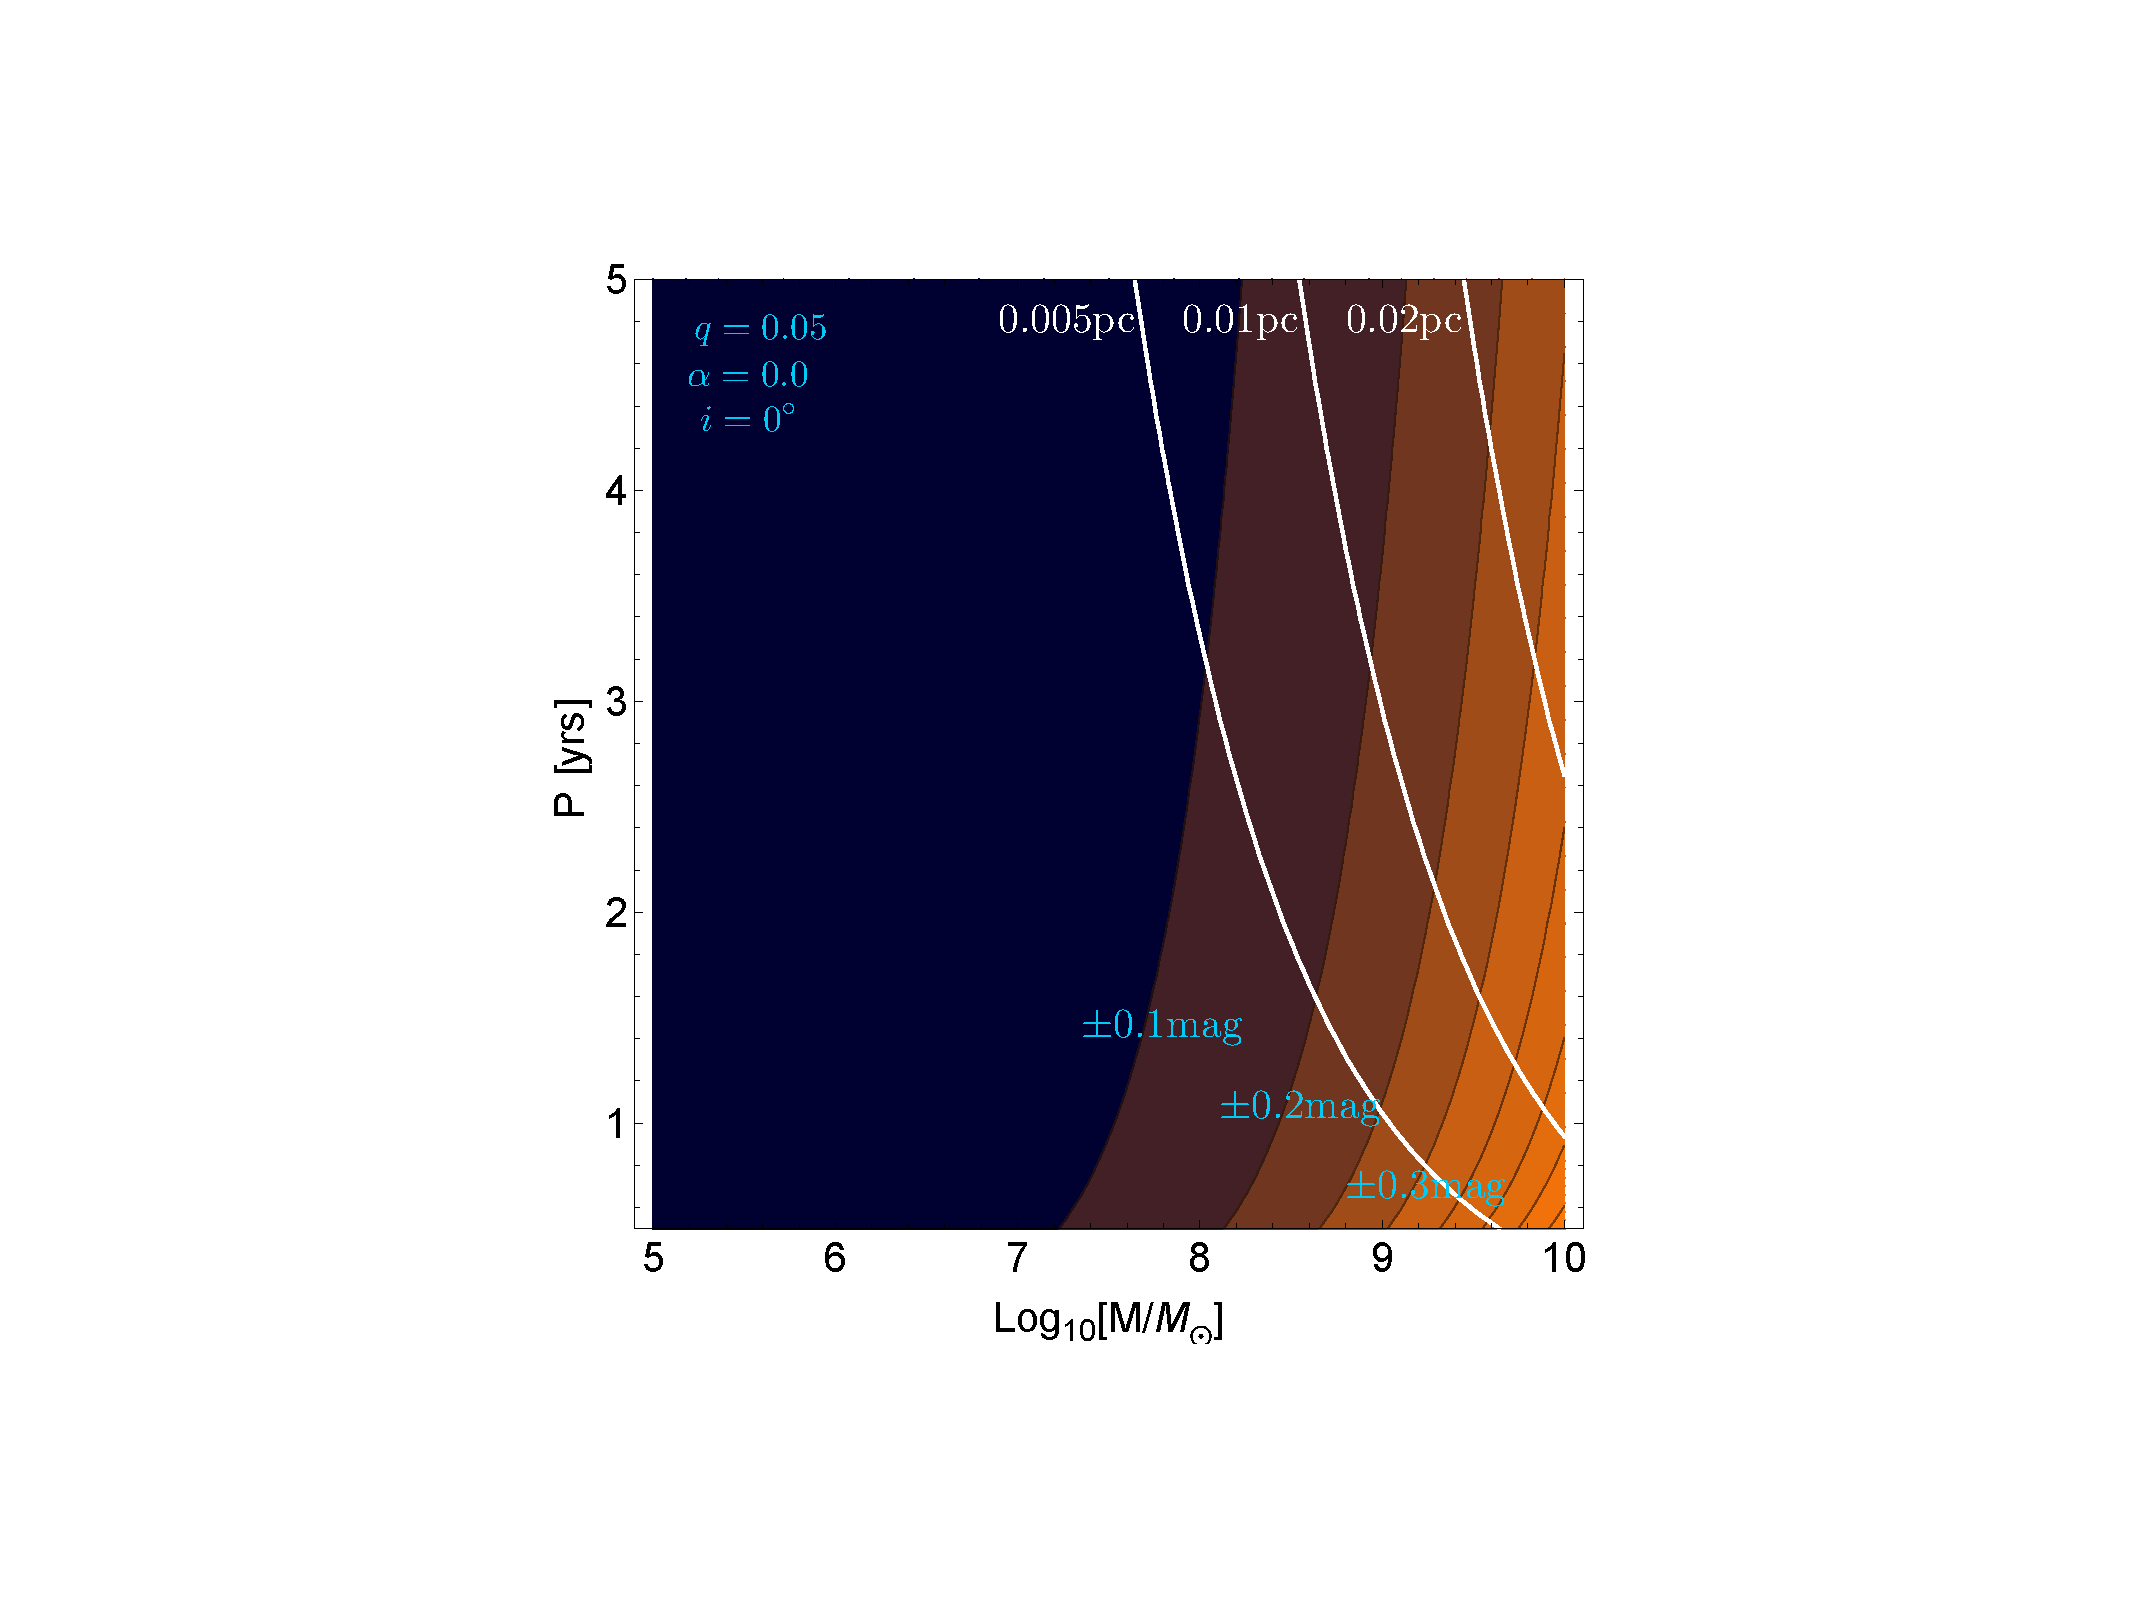
\includegraphics[scale=0.33]{figures/ch5/boosting_Pbin_M.pdf} \hspace{20pt} 
%
\end{array}$
\end{center}
\caption{Representative binary total masses and orbital periods for which
Doppler  boosting is an important cause of periodicity. Cyan contours draw
lines of constant Doppler modulation amplitude in magnitudes. White contours
are binary separations at the given orbital period and binary mass. Electric-green 
contours estimate the ratio of the light crossing time at the inner edge
of a dust distribution $t_d$ to the binary orbital period (see \S \ref{S:PDs}). 
We have assumed a mass ratio of $q=0.05$, an edge-on viewing of the
binary ($I=0.0$ rad), and a spectral index $\alpha=0.0$.}
\label{Fig:boostParams}
\end{figure}
%%%%%%%%%%%%%%%%%%%%%%%%%%%%%%%%%%%%%%%%%%%%%%%%



\section{Model derivation}
\label{S:Derivation}
\subsection{Isotropic emission from a central source}
\label{S:FISOderivation}

We first consider reverberation of UV/optical emission from the isotropic,
time-dependent central source. We assume that the dust is optically thick to
the UV/optical continuum source radiation and optically thin to its own
emission in the IR.


\subsubsection{Spherical dust shell}

We assume the source, with bolometric luminosity $L^{\rm iso}(t)$, is
surrounded by a sphere of dust with inner radius $\Rin$ where all of the
source emission is absorbed. We adopt spherical coordinates centered on the
dust shell ($r,\theta,\phi$), with the observer situated at coordinates $(r,
\theta, \phi) = (d, \pi/2, 0)$. The specific flux at the dust shell is
\begin{equation}
F^{\rm iso}_{\nu}(t, R_d) = \frac{L^{\rm iso}_{\nu}(t)}{4 \pi R^2_d}.
\end{equation}
This flux of continuum radiation heats the surrounding dust. By assuming that
the dust is in radiative equilibrium with the heating source, and given an
efficiency of absorption/emission by the dust $Q_{\nu}$, we find the dust
temperature as a function of time by equating the power absorbed by a dust
grain to that radiated,
\begin{eqnarray}
\pi a^2_{\eff}\bar{Q}^{\rm src}_{\nu} F^{\rm iso}(t, R_d) = 4\pi a^2_{\rm eff} \int^{\infty}_{0}{Q_{\nu} \pi B_{\nu}\left[T(t)\right] \ d \nu } ,
\label{Eq:TdISO}
\end{eqnarray}
where $a_{\rm eff}$ is the effective grain radius which describes the dust
cross section for absorption and also the surface area for emission, $\pi
B_{\nu}$ is the blackbody flux from a uniformly emitting dust grain at
temperature $T$, and $\bar{Q}^{\rm src}_{\nu}$ denotes an average over the
source spectrum.

Radiation with wavelength $\lambda = c/\nu \lsim 2 \pi a_{\eff}$ is absorbed
efficiently by dust grains. For longer wavelength radiation, grains of the
same size become transparent.  Hence for the absorption/emission efficiency we
choose $Q_{\nu}=1$ for frequencies above a cutoff $\nu_0 \sim c (2 \pi
a_{\eff})^{-1}$ and a power law fall off in efficiency for lower frequency
(long wavelength) radiation, $Q_{\nu} \equiv \rm{min}\left[ (\nu/\nu_0)^k,
1\right]$ where $k \geq 0$.\footnote{ For this form of $Q_{\nu}$, the right
hand side of Eq. (\ref{Eq:TdISO}) can be written in terms of polylogarithmic
functions.}  Because the efficiency for absorption is unity for high frequency
radiation, above $\sim$ $1\mu$m, we take $\bar{Q}^{\rm src}_{\nu} = 1$
throughout.


The observed flux due to one dust grain at temperature T is
\begin{eqnarray}
F^{\rm{grain}}_{\nu} &=& 2 \pi \int^{\theta_c}_0{ Q_{\nu} B_{\nu}(T) \cos{\theta_s} \sin{\theta_s} d \theta_s} = \left(\frac{ a_{\rm{eff}} }{d}\right)^2 Q_{\nu} \pi B_{\nu}(T) \\ \nonumber  
\theta_c &=& \sin^{-1}\left( \frac{ a_{\rm{eff}}}{d}\right) .
\end{eqnarray}
where $\theta_s = \theta_c$ is the angle subtended on the sky by a dust grain
with radius $ a_{\rm{eff}}$ at a distance $d$ from the observer. Given the
grain number density, the time dependent dust temperature everywhere in the
shell (Eq. (\ref{Eq:TdISO})), and assuming that dust is
optically thin to its own emission, we compute the total observed flux from
heated dust grains
\begin{eqnarray}
\label{Eq:FnuSS}
 F_{\nu}(t) &=& \left(\frac{ a_{\rm{eff}} }{d}\right)^2 \int^{2 \pi}_{0}{\int^{\pi}_{0}{ \Sigma_d Q_{\nu}  \pi B_{\nu}\left[T(t_{\em})\right]  R^2_d \sin{\theta} \ d \theta d\phi }}   \\ \nonumber 
 %
t_{\em}& =& t - \frac{\Rin}{c} \left( 1 - \sin{\theta} \cos{\phi}\right)  
\end{eqnarray}
where $\Sigma_d$ is the surface number density of the dust shell; $\Sigma_d
\rightarrow \pi^{-1} a^{-2}_{\eff}$ in the limit that all UV/optical radiation
is absorbed by the sphere. The most important aspect of the above equation is
that we have evaluated the temperature at the time $t_{\em}$; if light leaving
the front of the dust shell reaches an observer at time $t$, then light
emitted from the location ($\Rin$, $\theta$, $\phi$) reaches the observer at
time $t_{\em}$. By integrating over all locations in the dust shell at time
$t$, we take into account the finite light travel time. Put another way, we
evaluate the time changing dust temperature at the retarded time. The left
panel of Figure \ref{Fig:Schm} illustrates this by drawing cross sections of
the paraboloids of constant light travel time (described by the equation for
$t_{\em}$). Conceptually, the left panel of Figure \ref{Fig:Schm}, along with
the definition of $t_{\em}$, tells us that dust emission from a sphere of
radius $R_d$, at time $t$, is comprised of dust emission spanning a time
interval of $2 \Rin /c$ in the frame of the central emitting source. The
lesson being that the reprocessed dust emission is not necessarily a phase
shifted replica of the UV/optical emission. We revisit the role of $t_{\em}$
in \S \ref{S:Interp:Sphere}.


The total observed flux at an instrument with bandpass function $W(\nu)$ is
 \begin{equation}
F_{W}(t) = \int^{\infty}_{0}{  W(\nu) F_{\nu}(t) d \nu  } \sim \int^{\nu_{\rm max}}_{\nu_{\rm min}}{ F_{\nu}(t) d \nu}
\label{Eq:FISO}
 \end{equation}
where we assume that $W(\nu)$ is a top hat function with frequency
limits $\nu_{\rm min}$ and $\nu_{\rm max}$.



 %%%%%%%%%%%%%%%%%%%%%%%%%%%%%%%%%%%%%%%%%%%%%%%%
%%% FIGURE: Light Travel Geometry %%%
%%%%%%%%%%%%%%%%%%%%%%%%%%%%%%%%%%%%%%%%%%%%%%%%
\begin{figure}
\begin{center}$
\begin{array}{c c }
%
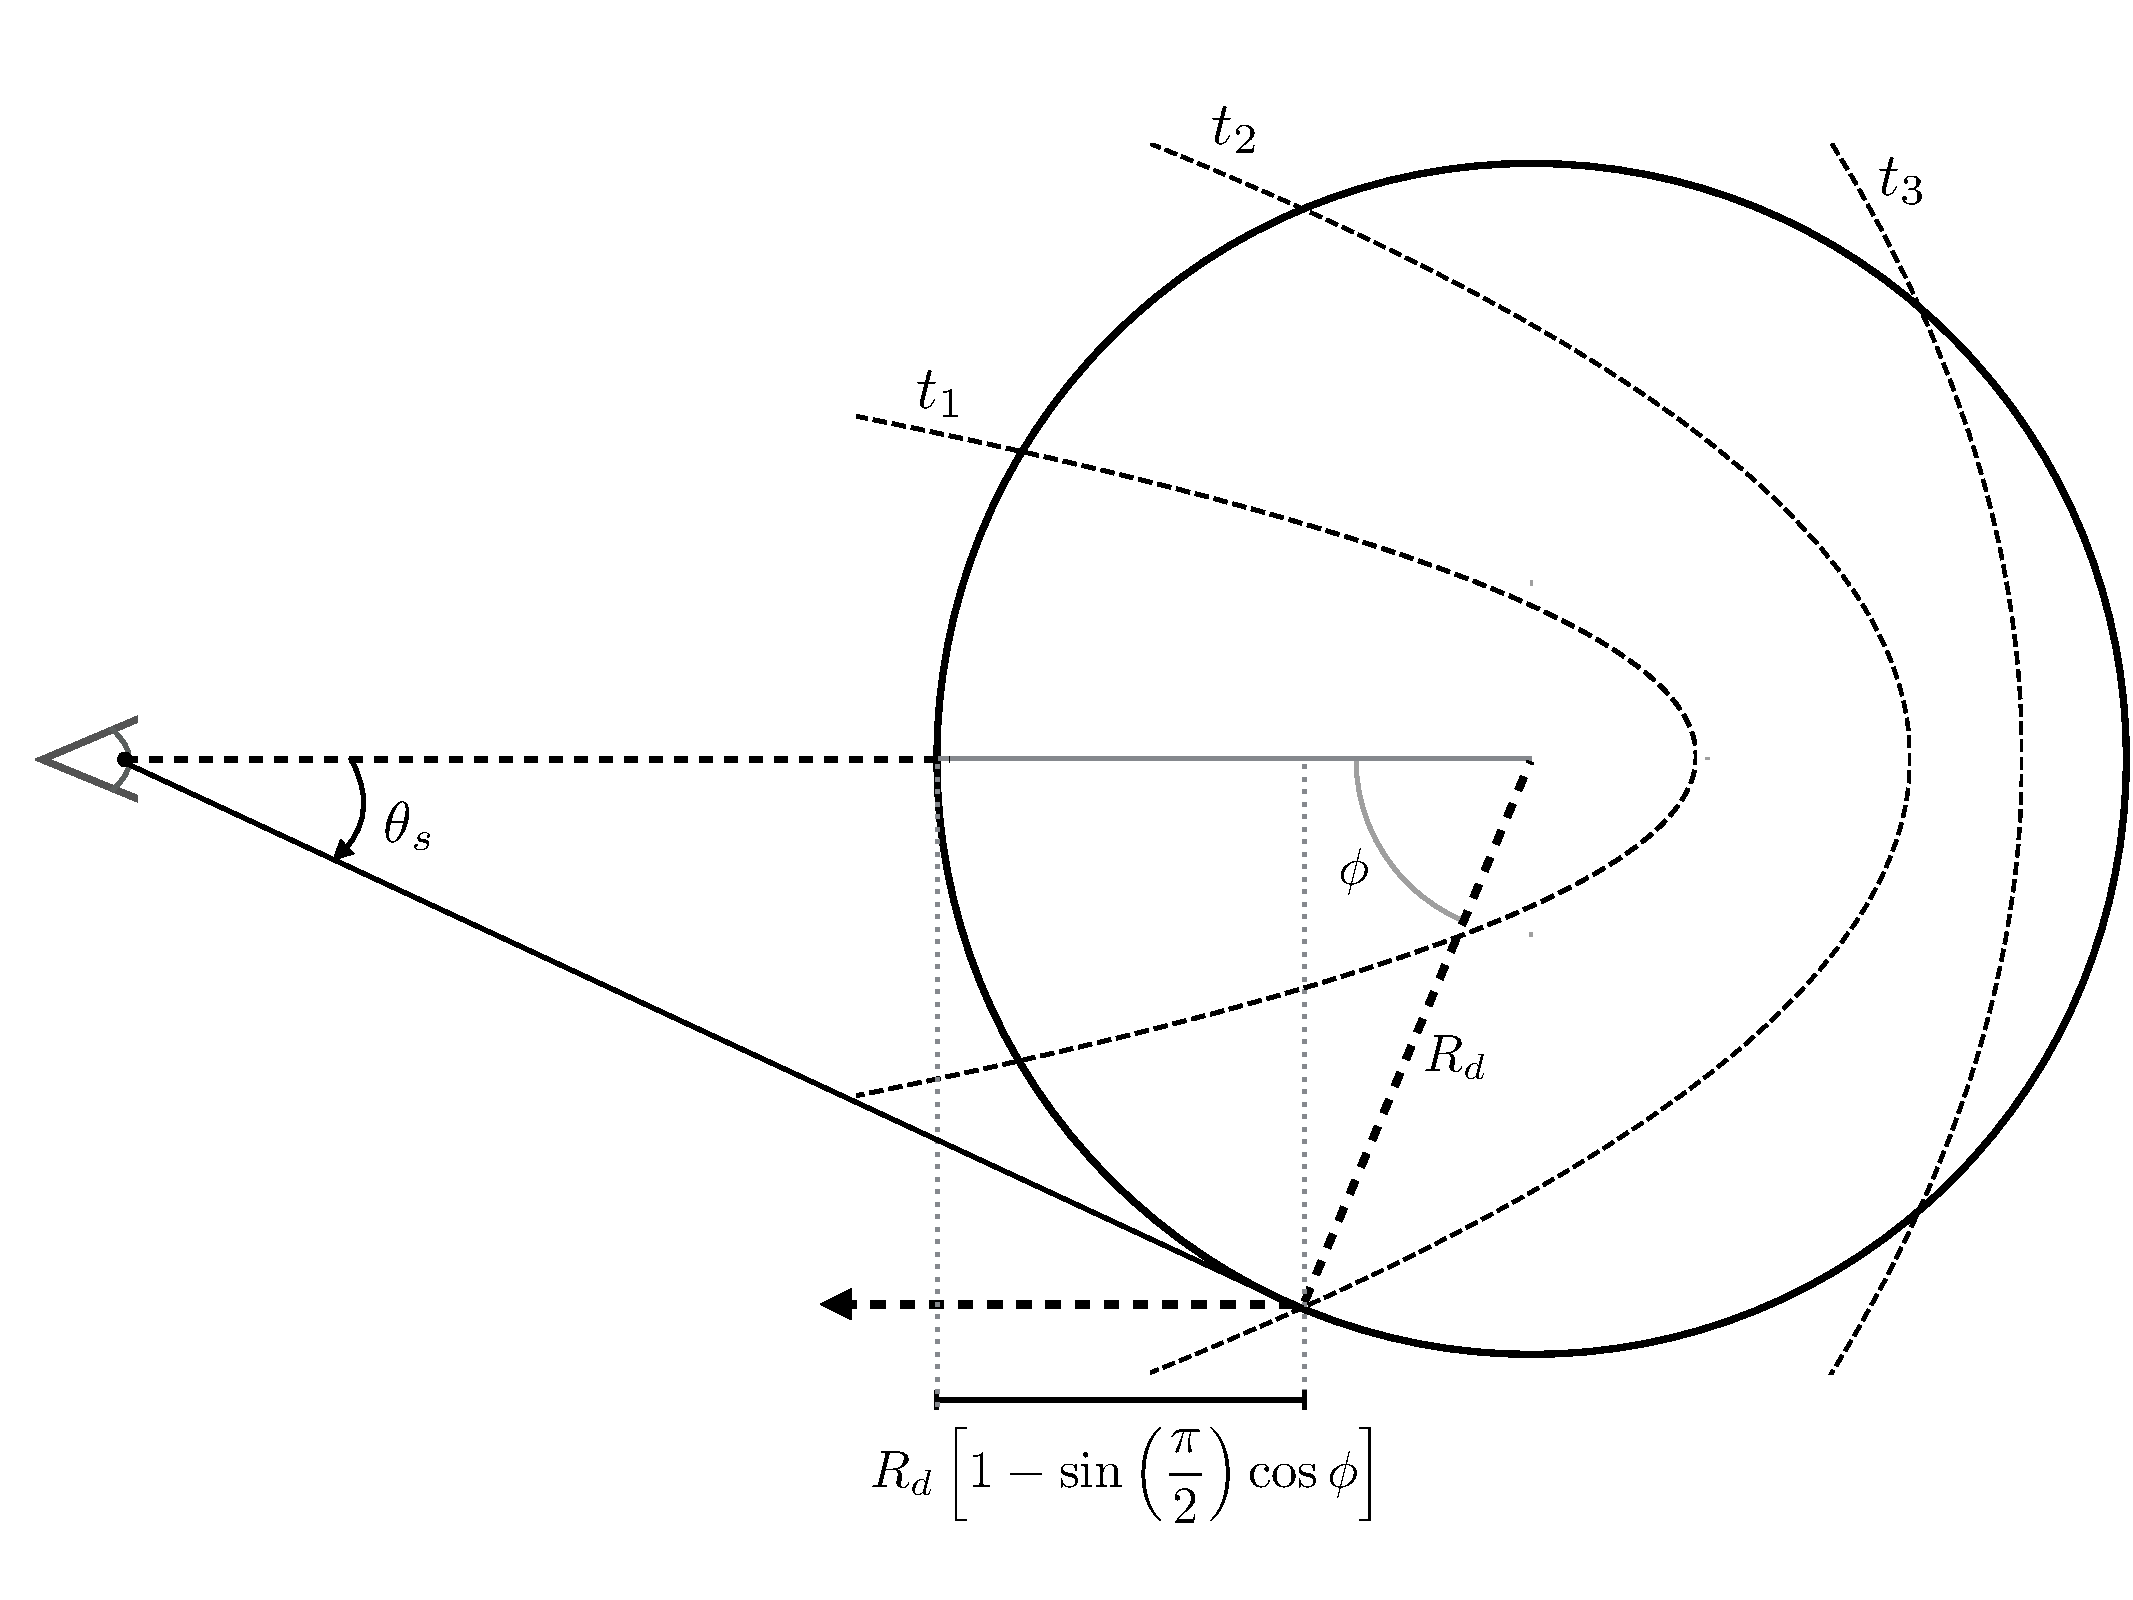
\includegraphics[scale=0.22]{figures/ch5/tem_schematic} \hspace{20pt} & 
 \includegraphics[scale=0.22]{figures/ch5/Torus_Schematic} 
%
\end{array}$
\end{center}
\caption{
Left: light travel time geometry: The circle is a cross section of an emitting
source. Light leaving the intersection of the emitting source and the parabola
$t_1$ reaches the observer before light leaving the intersections of the
source with $t_2$ and $t_3$. For a continuously emitting source, the
observer's instantaneous view consists of light summed over all past parabolas
intersecting the circle. Right: angles present in the torus geometry: $I$ is
the inclination of binary orbital plane to observer's line of sight, $J$ is
the inclination of torus axis to the plane perpendicular to the line of sight,
$\theta_T$ is the opening angle of the torus, and $\theta$ is the polar
spherical angle in our chosen coordinate system.
}
\label{Fig:Schm}
\end{figure}
%%%%%%%%%%%%%%%%%%%%%%%%%%%%%%%%%%%%%%%%%%%%%%%%








%%%%%%%
\subsubsection{Torus shell}
%%%%%%%

The dust sphere of the previous section has one geometric parameter, its
radius $R_d$. We expand upon the spherical model by cutting out portions of
the sphere to make an infinitely thin torus, or torus shell. Because we assume
the dust to be optically thick to UV/optical and optically thin to IR, such a
torus shell is equivalent to a torus or disc of finite radial extent because
only the inner edge absorbs UV/optical and then emits IR.


This introduces a
second and a third dust geometry parameter: the opening angle of the torus
$\theta_T$ and the inclination of the torus to the line of sight $J$. These
angles and the binary inclination angle are drawn schematically (for a torus
with finite radial extent) in the right panel of Figure \ref{Fig:Schm}. For
the torus model we simply set the temperature found in Eq. (\ref{Eq:TdISO}) to
zero for
\begin{eqnarray}
\theta'(J) < \theta_T \quad \rm{or} \quad \theta'(J) > \pi - \theta_T
\end{eqnarray}
where $\theta'(J)$ is the polar coordinate in a coordinate system rotated
around the y axis by angle $J$.














%%%%%%% 
\subsection{The Lighthouse: anisotropic, Doppler-boosted emission} 
%%%%%%% 
To include the effects of Doppler boosting in the IR light curve we only need
to change the form of the source (UV/optical) flux. From Eq. (\ref{Eq:Dop1}),
\begin{eqnarray}
F^{\rm{Dop}}_{\nu}(t, \Rin, \theta, \phi) %&=& \left[D(t, \theta, \phi)\right]^{3-\alpha_{\nu}} F^0_{\nu}(\Rin)  \nonumber \\
&=&  \left[D(t, \theta, \phi)\right]^{3-\alpha_{\nu}} \frac{L^0_{\nu}}{4 \pi R^2_d}  \\ \nonumber
D(t, \theta, \phi) &\equiv& \left[ \gamma \left(1 - \frac{v_{||}}{c} \right) \right]^{-1},
\label{Eq:DopFlux}
\end{eqnarray}
where $L^0_{\nu}$ is the rest frame, specific luminosity of the source,
$\gamma = \left[ 1 - (v_s/c)^2 \right]^{-1/2}$ is the Lorentz factor of the
secondary which orbits at speed $v_s = (1+q)^{-1}\sqrt{GM/a}$, $I$ is the
inclination angle of the binary's orbit to the line of sight, $\Omega$ is the
angular frequency of the binary and we assume throughout that the binary is on
a circular orbit. We continue to use the spherical coordinates as above with
($r,\theta, \phi$) centered on the binary center of mass and with the observer
situated at ($d,\pi/2$,0). We have approximated the distance from the
secondary to the dust shell as $\Rin$ (see Eq. (\ref{Eq:aORd}) below).

A key difference in this form of the Doppler formula and the usual form
presented by Eq. (\ref{Eq:Dop1}) is the line-of-sight velocity. Here the line of
sight velocity $v_{||}$ in the Doppler factor $D$ is the line of sight speed
of the secondary BH as observed by a dust grain at position
$\mathbf{\hat{r}}_{\rm{dust}}$ in the dust shell. Written in terms of
barycentric coordinates $(r,\theta, \phi)$,
\begin{eqnarray}
\label{Eq:vlos}
\frac{v_{||}}{c} &=& \frac{\mathbf{v_{s}} \cdot \mathbf{\hat{r}}_{\rm{dust}} }{c}\\ \nonumber 
& = & \beta  \left[ \cos{I} \sin{(\phi_0+\Omega t)} \sin{\theta}\cos{\phi} - \cos{(\phi_0+\Omega t)} \sin{\theta}\sin{\phi} - \sin{I} \sin{(\phi_0+\Omega t)} \cos{\theta}  \right],
\end{eqnarray}
where $\phi_0$ is the $\phi$ coordinate of the secondary at $t=0$ and we have
parameterized the secondary orbital velocity as $\beta \equiv a (1+q)^{-1}
\Omega$ which depends on the binary mass ratio $q$, total mass $M$, and period
$P$ through the binary orbital frequency $\Omega$ and separation $a$. The
Doppler case introduces three new source parameters $\alpha_{\nu}$, $\beta,$
and $I$ (taking the place of $A$ in the isotropic case).

Just as for the isotropically emitting source, we determine the temperature of
each patch of the dust shell by assuming radiative equilibrium between the
incident UV/optical flux and the dust. The difference here is that the
incident flux and resulting dust temperature are now spatially varying across
the sphere. The analogue of Eq. (\ref{Eq:TdISO}) becomes
\begin{equation}
\label{Eq:TdDop1}
\bar{Q}_{\nu} \int^{\infty}_{0}{F^{\rm{Dop}}_{\nu}(t, R_d, \theta, \phi)  \ d \nu } =   4 \int^{\infty}_{0}{Q_{\nu} \pi B_{\nu}\left[T(t,\theta, \phi)\right] \ d\nu}.
\end{equation}
We approximate the LHS of the above equation as
\begin{equation}
\label{Eq:TdDop}
\left[D(t, \theta, \phi)\right]^{3-\bar{\alpha}} \frac{L^0}{4 \pi R^2_d}  =   4 \int^{\infty}_{0}{Q_{\nu} \pi B_{\nu}\left[T(t,\theta, \phi)\right] \ d\nu}. 
\end{equation}
where $L^0$ is the bolometric source luminosity and we have approximated the
frequency dependent source spectral slope $\alpha_{\nu}$ by an average over
source frequency $\bar{\alpha}$. This solution for the dust temperature can be
used in either of the solutions for $F_{\nu}$ derived for an isotropic source
in \S \ref{S:FISOderivation}.










\section{Analysis}
\label{S:PDs}

We now identify the effect of the model parameters (Table \ref{Table:params})
on the IR light curves. For the purposes of comparing to continuum light
curves and their reverberated IR counterparts, the interesting features of the
reverberated light curve are the average brightness, phase, and
variability amplitude relative to the UV/optical continuum.

In the general case we compute IR light curves by numerically solving for the
dust temperature in Eqs. (\ref{Eq:TdISO}) or (\ref{Eq:TdDop}) and then
evaluating Eqs. (\ref{Eq:FnuSS}) and (\ref{Eq:FISO}) for the total in-band
flux. We first build up intuition for reverberation of periodic sources by
analytically evaluating simplified cases.








\begin{table}
%
\rotatebox{90}{
%
%\begin{center}
\begin{tabular}{ c | c | c | c}
        Parameter         & Meaning     & Fiducial Value   &   Notes \\
                   \hline 
                  Source Parameters &  & \\
                  \hline    
$L^0$ \quad    & Bolometric source luminosity            & $6.78\times10^{46}$  erg s$^{-1}$    & PG 1302 value\\
%
%$M$                                     & Total Mass        & $10^{9.1} \rightarrow 10^{9.4} \Msun $      \\
$P$  \quad     & Variability period                        & $R_d /c$   & Binary orbital period for Doppler\\
%
%Doppler &&& \\
$\bar{\alpha}$     & Source averaged spectral index            &  0.0  & Doppler source parameter \\
%$q$                                       & Mass ratio           & $\lsim 0.1$    \\
$\beta$             & Boost velocity$/c$                       & $0.068$   & PG 1302 value \\
&&& Inferred from binary mass,\\
&&& period, and mass ratio. \\
$I$                 & Inclination                          &  $0$  & Doppler source parameter \\
&&& $0$ is edge-on \\%Inferred from $\beta$ and variability magnitude   \\
                   \hline   
                  Dust Parameters &  & \\
                  \hline    
$\Rin$               &  Inner edge of dust                                      & $\chi R_0 = \chi 0.9 \sqrt{\epsilon/0.1}$ pc      & $R_0=$Sublimation radius for \\
&&& Graphites around PG 1302\\
%{$n_0$}            &  Density normalization                                 & $(p-1) (\pi a^2_{\eff} \Rin)^{-1}$    &       \\
%{$p$}                &  Density exponent                                    & 2.0                       &   $n_d(r) = n_0 \left( \Rin/r \right)^{p}$    \\
{$J$}                &  Torus inclination                                       & $\pi/2$                       &   0 obscured; $\pi/2$ unobscured \\
{$\theta_T$}     &  Torus opening angle                                   & $\pi/4$                     &   0 is a dust sphere\\
%$\Rout$            &  Outer edge of dust                                   & $10\Rout$                     & weak dependence for $p>0$     \\
$k$             &  Absorption/emission efficiency exponent                      & 1                             &   \\
$\nu_0$     & Efficiency cutoff frequency                           &    $c/(2 \pi a_{\rm{eff}})$           & $Q_{\nu} = \rm{min}\left[ \left( \nu/ \nu_0 \right)^{k}, 1\right]$    \\
$a_{\rm{eff}}$  &  Grain size                                               &  $0.16$ $\mu$m                    &  Set by $\nu_0$       
 \end{tabular}
 %
 }
 \caption{Parameters of the model and their fiducial values if not otherwise stated in the text.}
 %
%\end{center}
\label{Table:params}
%\thispagestyle{empty}
\end{table}










\subsection{Spherical dust shell} 
\label{S:Interp:Sphere} 

\subsubsection{Simplest case}
For demonstrative reasons, we first consider the simplest case: isotropic,
sinusoidal emission by the central source, and ignore light travel time
effects as well as dust absorption/emission efficiency ($Q_{\nu} \rightarrow
1$). In this case, the dust temperature is observed to be constant across the
dust sphere at a given time,
\begin{equation}
T^4(t) =  \frac{L(t)}{16 \pi R^2_d \sigma},
\end{equation}
where $L(t)$ is the time variable continuum (UV/optical) emission from 
the central illuminating source, and $\sigma$
is the Stephan-Boltzmann constant. The IR luminosity of one grain is simply $4
\pi a^2_{\eff} \sigma T^4$ and the total IR luminosity is found by
multiplying by the number of grains, $\Sigma_d 4 \pi R^2_d$, then
\begin{equation}
L_{\rm{IR}}(t) =  \Sigma_d \pi a^2_{\eff} L(t) \rightarrow L(t)
\end{equation}
where the $\rightarrow$ holds in the limit that  $\tau  \rightarrow 1$  so
that $\Sigma_d \rightarrow \pi^{-1} a^{-2}_{\eff}$. When light travel time is
ignored, the IR light curves should track exactly the UV/optical light curves; we
confirm this to be the case in our numerical scheme for solving the equations
of \S \ref{S:Derivation} by setting $Q_{\nu} = 1$ and $t_{\em} = t$ and finding
agreement of IR and UV/optical light curves, as we must.

\subsubsection{Time delays}
Re-introducing the time delay, the assumption that $T$ is observed to be
constant across the sphere breaks down even in the isotropic case. The IR
luminosity evaluated at the retarded time $t_{\em}$ (Eq. (\ref{Eq:FnuSS})),
integrated over all frequencies, becomes
\begin{eqnarray}
L^{\rm{Iso}}_{\rm{IR}}(t)
&=&\Sigma_d 4 \pi a^2_{\eff} \int^{2 \pi}_0{\int^{\pi}_0{  \frac{L\left( t_{\em}(t, \theta, \phi) \right)}{16 \pi R^2_d } R^2_d \sin{\theta} d\theta d\phi }} \nonumber \\
&=&  \Sigma_d \pi  a^2_{\eff} L^0  \left[ 
  1 +  A \rm{sinc}{\left( \Omega t_d \right)}  \sin{ \left( \Omega \left( t - t_d \right) \right)  }
   \right],
   \label{Eq:LIR_sp}
\end{eqnarray}
for which the last line follows only if we rotate our coordinate 
system so that the observer is looking down the z-axis (instead of the x-axis) 
or equivalently if $J= \pi/2$). Here $\rm{sinc}(x) = \sin{x}/x$ is the 
cardinal sine function, and we assumed the UV/optical luminosity of 
Eq. (\ref{Eq:Fsrc_ISO}),
\begin{equation}
L(t) =  L^0  \left[ 
  1 +  A \  \sin{ \left( \Omega t  \right)  }
   \right].
\end{equation}
with average luminosity $L^0$ and amplitude of modulation $A$.\footnote{This
analytic results can be generalized to arbitrary periodic functions by
replacing $L(t)$ with a Fourier series expansion.}

From this simple expression we learn a great deal about reverberation of
periodic continuum. First, we find, as expected, that the average luminosity
of the UV/optical emission, in the case where the dust is optically thick to
continuum emission, is the same as the average luminosity of the IR. 
What we find that is new, is that the amplitude of modulation is
necessarily diminished by a factor,
\begin{eqnarray}
\frac{A^{\rm{Iso}}_{\rm{IR}}}{A} = \frac{1}{2 \pi}\frac{P}{t_d} \sin{\left[ 2 \pi\frac{t_d}{P} \right]},
\label{Eq:AIRoAUV}
\end{eqnarray}
where $A_{\rm{IR}}$ is the amplitude of IR modulation, $A$ is the amplitude of
UV/optical modulation, we have defined $t_d \equiv R_d/c$, and $P = 2 \pi
/\Omega$, the period of the varying source.  We find also that the IR is
modulated at the same period as the UV/optical continuum, but with a phase lag
given by
\begin{eqnarray}
\Phi_{\rm{Iso}} &=& \frac{t_d}{P} -  \left[1 - \rm{sign}\left(\frac{A^{\rm{Iso}}_{\rm{IR}}}{A}\right) \right] \frac{1}{4}  \quad \rm{cycles}
\label{Eq:ISOLags}
\end{eqnarray}
written in fractions of a cycle. When the IR amplitude (\ref{Eq:AIRoAUV}) is
positive, we recover the expected phase lag given by the light travel time
from the central source to the dust shell. However, if $A_{\rm{IR}} < 0$, there
is an additional $1/2$ cycle phase change discussed below. We stress that this
half-cycle phase change is only pertinent for sources that are reflection 
symmetric about their average.




Eq. (\ref{Eq:AIRoAUV}) tells us that the amplitude of IR modulation is
determined by the ratio $t_d/P$. For $t_d/P \rightarrow 0$ the IR amplitude
matches the UV/optical amplitude. As $t_d/P$ increases, the relative IR to
UV/optical amplitude decreases, falling to  zero amplitude at $t_d/P  \gg 1$
and at the values where $t_d/P = \frac{m}{2}$. The analytic result Eq.
(\ref{Eq:LIR_sp}) is depicted in Figure \ref{Fig:AIRoAUV_sp}, along with the
results of our numerical calculation of the corresponding expressions in \S
\ref{S:Derivation}. Integrating over all frequencies, we find the expected
agreement between analytic and numerical results.





%THE BELOW REASONING IS DIFFERENT (ITHINK) FROM WHY THE PERIODIC SOURCE HAS LOWER AMPLITUDE FOR LARGER TD/P in the periodic case, more periods fill the sphere and the so remainder which causes non-zero amplitude gets smaller. For the flare case, the same energy is distributed over a longer time as td->P

% That the amplitude of IR variations drops to zero for $t_d \gg P$ is expected
% even for a non-periodic source. If $P$ were instead the characteristic
% timescale for flare-like emission, then $\sim t_d + P$ is the timescale for IR
% light to reach us from the entire sphere and $(t_d+P)/P$ sets the ratio of
% emission timescales in IR to UV/optical. Since the energy emitted in the IR,
% $E_{\rm{IR}}$, is less than or equal to the energy emitted in the UV/optical,
% then the luminosity flare in the IR reaches a characteristic luminosity:
% $L_{\rm{IR}} \sim E_{\rm{IR}}/(t_d+P)$, and because $L^0 \sim E^0/P$, then
% $L_{\rm IR} \lsim L^0 P/(t_d+P)$.






The condition for zero IR amplitude, $t_d/P = \frac{m}{2}$, for an isotropic,
periodic continuum source is the condition that the light crossing time of the
dust shell is an integer multiple of the variability period. Because the
temporal variation of the source is sinusoidal, finite light travel time
causes the observed spatial variation of temperature (and hence grain flux)
across the dust shell to also be sinusoidal. Then at time $t_0$ the dust
temperature ranges from $T(t_0)$ at the front of the sphere to $T(t_0 - 2t_d)$
at the back of the sphere. With $t_d = \frac{m}{2}P$, the back of the sphere
and the front are the same temperature with $m$ sinusoid periods of flux
variation in between. As time increases to $t > t_0$ this does not change and
neither does the integrated flux over the entire sphere.


%DD: this explanation has some confusing points still - why does the integer mult of cycles cause constant luminosity if the peaks and troughs change position on the sphere in time?

When $t_d/P \neq \frac{m}{2}$, a non-integer fraction of a variability cycle
is observed at once across the dust shell. The total luminosity in the non-
integer remainder sets the amplitude of IR variability. To understand this
further, imagine we are looking down the z-axis of the sphere, and that we can
resolve the luminosity structure of the dust sphere; each $x-y$ cross section
emits a different luminosity corresponding to different times in the source's
past. IR luminosity variations in time occur because the location of the non-
integer remainder marches steadily backwards in the $-z$ direction, in $x-y$
annuli over the surface of the sphere. The $z$ location of the remainder sets
the size of the emitting region and hence the total luminosity attributable to
the non-integer remainder; the result is a sinusoidal variation about the
mean. IR light curves for which the remainder is dimmer than the mean are
inverted about the mean compared to IR light curves for which the remainder is
hotter than the mean, hence the half-cycle phase change found mathematically
(see the discussion after Eq. (\ref{Eq:ISOLags}). When the remainder is in
between a half-integer and a whole-integer number of cycles, it consists of
the negative part of the sine wave and is dimmer than the mean. The remainder
is brighter than the mean when the it is in between a whole-integer and a
half-integer cycle, consistent with Figure \ref{Fig:AIRoAUV_sp}. By this
reasoning, the maximum amplitude modulations occur when the remainder is
approximately one quarter of a cycle, which is also what we find
mathematically. For $t_d \gg 1$, the non-integer remainder is a smaller
fraction of the entire luminosity emanating from the sphere (more full cycles
fit within one dust light crossing time), hence the amplitude of IR
variability decreases with larger $t_d/P$, as found in Figure
\ref{Fig:AIRoAUV_sp}.






%%%%%%%%%%%%%%%%%%%%%%%%%%%%%%%%%%%%%%%%%%%%%%%%
%%% FIGURE: Sphere amplitude ISO vs Dop%%%
%%%%%%%%%%%%%%%%%%%%%%%%%%%%%%%%%%%%%%%%%%%%%%%%
\begin{figure}
\begin{center}
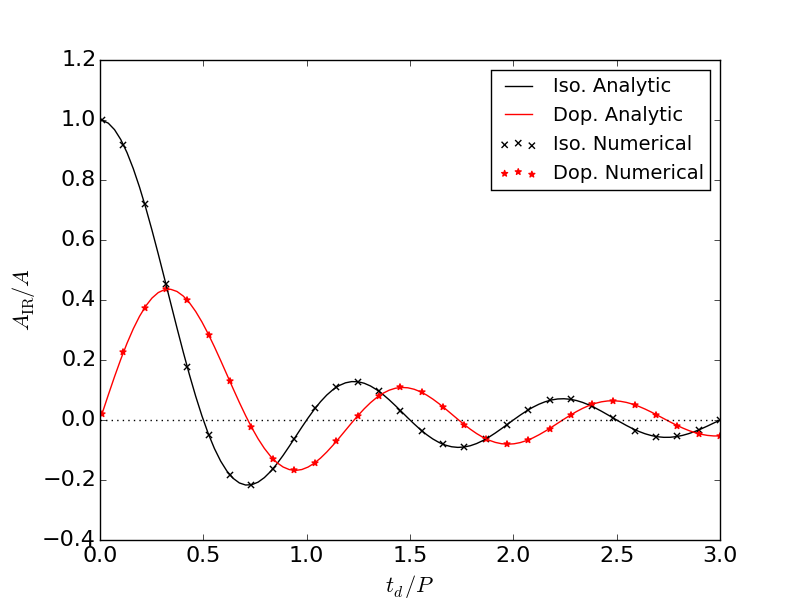
\includegraphics[scale=0.33]{figures/ch5/AIRplots/DopvsISO_AIRoAUV_alpha4_TsubCut1800_J1p5708_numin0_numx3_reclim50_TRHS2mx}
\end{center}
%
\caption{The fractional amplitude of IR variability $A_{\rm{IR}} = \Delta
L_{\rm{IR}}/L_{\rm{IR}}$ relative to the UV/optical amplitude $A=\Delta L/L$ for a
spherical dust shell which absorbs all UV/optical radiation and emits
it all in IR. The IR amplitude is given by the absolute value of the plotted
quantity while positive and negative values denote a half cycle phase
difference. Numerical values, for both isotropic (black x's) and
Doppler (red stars) sources, are computed from the peaks and troughs of
solutions for IR light curves laid out in \S \ref{S:Derivation}. The analytic
solutions (solid lines) are Eq. (\ref{Eq:LIR_sp}) for the isotropically varying
source (black) and Eq. (\ref{Eq:LIR_Dop_sp}) for the specific case of a
Doppler source with $\alpha_{\nu}=4$ and $v/c \ll 1$.} 
%
\label{Fig:AIRoAUV_sp}
\end{figure}
%%%%%%%%%%%%%%%%%%%%%%%%%%%%%%%%%%%%%%%%%%%%%%%%
%%%%%%%%%%%%%%%%%%%%%%%%%%%%%%%%%%%%%%%%%%%%%%%%
%%%%%%%%%%%%%%%%%%%%%%%%%%%%%%%%%%%%%%%%%%%%%%%%



\subsubsection{Doppler Source} 

When $v/c$ is small, and choosing $\alpha_{\nu}=4$, the relativistic Doppler
factor in Eq. (\ref{Eq:DopFlux}) can be written $D \sim 1 - v_{||}/c$. In this
approximation, the IR luminosity in the case of a Doppler-boosted source is
\begin{equation}
L^{\rm{Dop}}_{\rm{IR}} =  \Sigma_d \pi  a^2_{\eff} L^0 \left[ 
  1 +  \beta \cos{I} \left[ \frac{ \sin{\Omega t_d} }{\Omega^2 t^2_d} - 
  \frac{\cos{\Omega t_d}}{\Omega t_d}\right] \cos\left( \Omega \left( t - t_d\right)\right)
   \right],
   \label{Eq:LIR_Dop_sp}
\end{equation}
where there is an $\alpha$ dependence in the general case. 




Eq. (\ref{Eq:vlos}) tells us that the observer sees a UV/optical continuum
variation of the form $\sin\left( \Omega t\right)$ while the reverberated IR
variation is of the form $\cos\left( \Omega \left( t - t_d\right)\right)$.
This means that the reverberated Doppler solution exhibits a 
\begin{equation}
\Phi_{\rm{Dop}} = \frac{t_d}{P} - \rm{sign}\left(\frac{A^{\rm{Dop}}_{\rm{IR}}}{A} \right) \frac{1}{4} \quad \rm{cycles}
\label{Eq:DOPLags}
\end{equation}
lag; the Doppler IR light curves are a quarter cycle out of phase
with the isotropic case. This can be understood in analogy
to the isotropic case, where the IR is delayed by the light travel time
difference between the front of the sphere and the cross section half way
between front and back ($\phi = \pi/2$ and  $t_{\em} = t-R_d/c$ in
Figure \ref{Fig:Schm}). This is also the case for the Doppler source, however,
the Doppler flux seen by dust at $\phi = \pi/2$ is one quarter of a cycle
out of phase from the Doppler flux seen by the observer at $\phi = 0$. For
example, when the secondary BH is moving towards the observer line of
sight, the observer sees the maximum optical flux, but the dust at $\phi =
\pi/2$ sees the average flux - one quarter cycle difference.

 

The relative amplitudes also differ from the isotropic case,
\begin{equation}
\frac{A^{\rm{Dop}}_{\rm{IR}}}{\beta \cos{I}}  =  \frac{ \rm{sinc}{ \left( 2 \pi \frac{t_d}{P} \right)  }    }{2 \pi \frac{t_d}{P}}
 -   \frac{\cos{ \left(2 \pi \frac{t_d}{P}  \right) } }{ 2 \pi \frac{t_d}{P} }
  \label{Eq:DopAIR_sp}
\end{equation}
 where we have replaced A of the isotropic case with the Doppler analogue $\beta \cos{I}$. It is interesting to note that in this approximation, $A^{\rm{Dop}}_{\rm{IR}}$ is the negative derivative, with respect to $2 \pi t_d/P$, of $A^{\rm{Iso}}_{\rm{IR}}$; we are not aware of this being anything more than a mathematical coincidence.


Figure \ref{Fig:AIRoAUV_sp} plots the relative IR-variability amplitudes using
the analytic result for the Doppler-boosted source (Eq.
(\ref{Eq:LIR_Dop_sp})).  Figure \ref{Fig:AIRoAUV_sp} also plots results of the
numerical calculation using the  expressions derived in \S \ref{S:Derivation},
in the limit that Eq. (\ref{Eq:LIR_Dop_sp}) was derived. The amplitude of
modulations for the Doppler case falls to zero for $t_d/P \rightarrow 0$ where
as, in the same limit of the isotropic case, the IR modulation increases in
amplitude to match the UV/optical amplitude. The difference is rooted in the
nature of the source variability for the two cases. Because the Doppler-
boosted emission is observer dependent, and emanating from a steady rest-frame
source, conservation of energy requires that the total emission integrated
over a sphere does not vary in time (even though an observer at each point on
the sphere sees a varying flux). Observed IR variability arises because finite
light travel times from each part of the sphere cause the observer to see each
cross section, in the plane perpendicular to the observer, heated at different
times in the source evolution (see Figure \ref{Fig:Schm}), this changes as the
rotating lighthouse pattern of the Doppler-boosted source varies from front to
back of the dust sphere. As $t_d/P \rightarrow 0$, the time delay becomes
insignificant and the observed IR amplitude falls to zero.



%zeros of Doppler curve
Figure \ref{Fig:AIRoAUV_sp} shows that the Doppler IR emission has zero
variability amplitude at values of $t_d/P$ which are offset, also by
approximately one quarter cycle, from the analogous nodes of the isotropic
case. For a Doppler-boosted source, the zero amplitude solutions
and the maximum amplitude solutions are given by the values of $t_d/P$ for
which
\begin{equation}
2 \pi \frac{t_d}{P} = \tan{2 \pi \frac{t_d}{P}}.
\label{Eq:DopZeros}
\end{equation}
The first zero amplitude is at $\Omega t_d = 2 \pi t_d/P = 0$; the others are approximated by
\begin{equation}
\left. \frac{t_d}{P} \right|_{\rm{zeros}} \approx  \frac{2m + 1}{4} - \frac{1}{\pi^2 (2m+1)}   \qquad m=1,2,3... .
%\label{Eq:DopZeros}
\end{equation}
which converges to the condition that $t_d \approx \left( \frac{m}{2} +
\frac{1}{4}\right) P$ for $t_d \gg P$.

The largest Doppler IR amplitudes occur where 
\begin{equation}
\frac{2 \Omega t_d}{(\Omega t_d)^2 -2} =  \tan{\Omega t_d},
\label{Eq:DopExtrm}
\end{equation}
with its first three solutions at $\Omega t_d = 2 \pi t_d/P \approx 0.33, 0.95,
1.46$ and subsequent solutions approaching $t_d/P = m/2$, $m=4,5,6...$ the
zeros of the isotropic case. \footnote{This of course follows because of the
derivative relation between the Doppler and Isotropic amplitudes (see
discussion below Eq. (\ref{Eq:DopAIR_sp}))}




In deriving Eq. (\ref{Eq:LIR_Dop_sp}), we assumed that $\alpha_{\nu}=4$. The
dependence on $\alpha$ is shown numerically in Figure \ref{Fig:Dop_alph}. For
$\bar{\alpha} > 4$ the relative IR amplitude increases, while for $\bar{\alpha} < 4$, the
IR amplitude decreases relative to the UV. The largest differences are at the
peak IR amplitudes (Eq. (\ref{Eq:DopExtrm})).
%DD Is there a conceptual reason for this alpha dependence?


%%%%%%%%%%%%%%%%%%%%%%%%%%%%%%%%%%%%%%%%%%%%%%%%
%%% FIGURE: Dop_alpha Figure
%%%%%%%%%%%%%%%%%%%%%%%%%%%%%%%%%%%%%%%%%%%%%%%%
\begin{figure}
\begin{center}
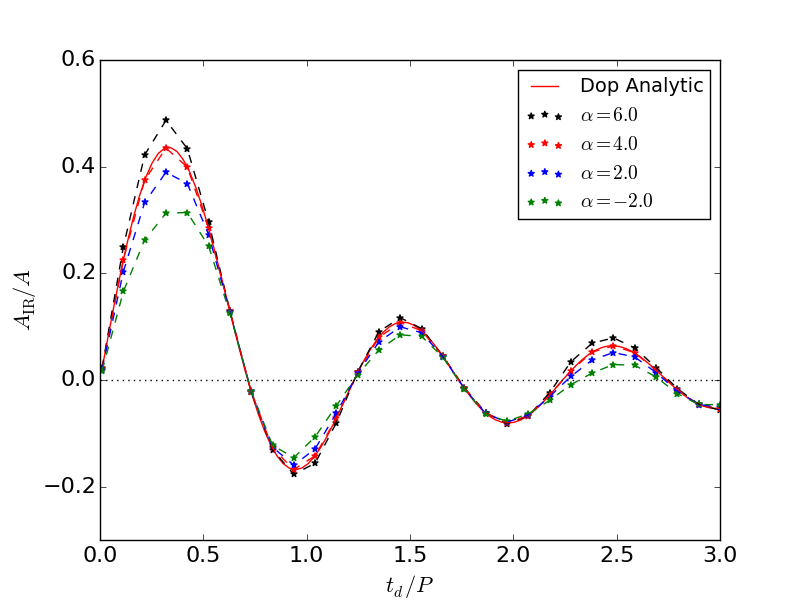
\includegraphics[scale=0.33]{figures/ch5/AIRplots/DopvsAlpha_AIRoAUV_J1p5708_numin0_numx5_reclim2_TRHS}
\end{center}
%
\caption{The same as Figure \ref{Fig:AIRoAUV_sp}, but for a Doppler source
with various values of the source spectral index $\alpha_{\nu}$. The analytic
solution Eq. (\ref{Eq:LIR_Dop_sp}) is for $\alpha=4$. Here $\nu_{\mu m}$ is 
the frequency of one $\mu$m radiation.}
%
\label{Fig:Dop_alph}
\end{figure}
%%%%%%%%%%%%%%%%%%%%%%%%%%%%%%%%%%%%%%%%%%%%%%%%



%Absorption 
\subsubsection{Absorption/emission efficiency}

We have so far ignored the efficiency of dust absorption and emission
$Q_{\nu}$. In the limit of our analytic solutions for the IR luminosity, where
we integrate over all frequencies, dust absorption/emission does not affect
our result. This is simple to see from Eq. (\ref{Eq:TdISO}) or Eq.
(\ref{Eq:TdDop}), where the r.h.s. integrand can be an arbitrary function of
$\nu$ as long as integration is taken over all frequencies in the calculation
of the reverberated IR flux (Eq. \ref{Eq:FISO}). However, when integrating
over a specific wave band, the variation in dust temperature shifts the dust
spectrum blue-ward and red-ward over a variability cycle. This can cause an
extra source of instrument dependent IR variability not considered so far.
This band specific variability depends on the absorption/emission efficiency
of the dust, and specifically where the cutoff in efficiency occurs relative
to the observing band.

Figure \ref{Fig:Qvon} shows the affects of including dust absorption/emission
efficiency and a finite frequency band. Figure \ref{Fig:Qvon} plots the
analytic solution and compares with numerical solutions that integrate over a
narrow range of frequencies from $2.8\mu$m to $4.0\mu$m (the WISE W1 band). In
Figure \ref{Fig:Qvon}  we choose $Q_{\nu} = \rm{min}\left[ \left( \nu/ \nu_0
\right)^{k}, 1\right]$ with $k=10$ and three different $\nu_0$ at the center
and edges of the W1 band. Even with this extreme spectral cutoff in the
observing window, the small temperature changes are not enough to shift the
dust spectrum across the observing band and boost IR variability, instead we
see that the effect of narrowing the observing band (from all frequencies) is
to decrease the relative IR variability amplitude.

%DD: why does it decrease?






%%%%%%%%%%%%%%%%%%%%%%%%%%%%%%%%%%%%%%%%%%%%%%%%
%%% FIGURE: AIR with Dust eff%%%
%%%%%%%%%%%%%%%%%%%%%%%%%%%%%%%%%%%%%%%%%%%%%%%%
\begin{figure}
\begin{center}$
\begin{array}{c}
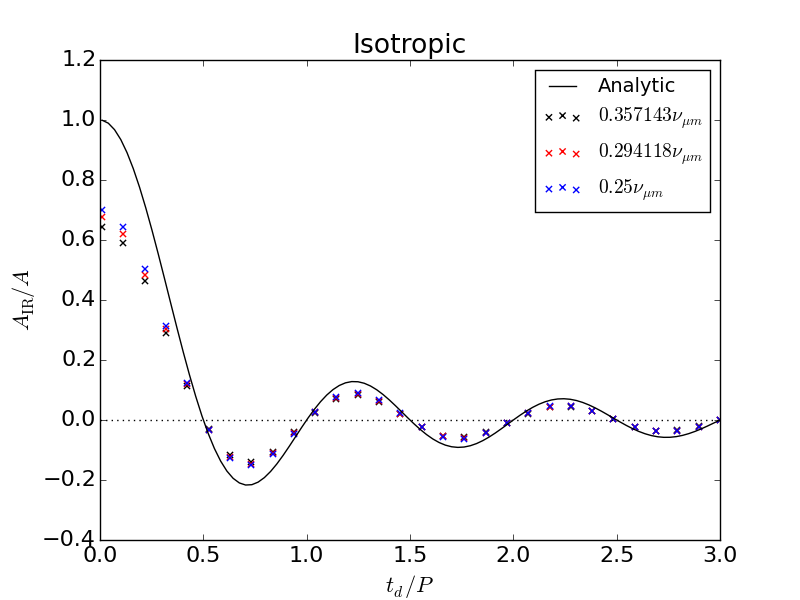
\includegraphics[scale=0.33]{figures/ch5/AIRplots/Qv_varnu0_SublimationCutT3000_AIRoAUV_k10_J1p5708_numin0p357143_numx0p25_reclim2.png} 
\end{array}$
\end{center}
%
\caption{
The same as Figure \ref{Fig:AIRoAUV_sp} except showing the effect of
integrating over a finite wave band. Even an extreme choice of $Q_{\nu}$
($k=10$ and the labeled cutoff frequencies in the the observing band) only
slightly diminishes the IR variability amplitude.
}
%
\label{Fig:Qvon}
\end{figure}
%%%%%%%%%%%%%%%%%%%%%%%%%%%%%%%%%%%%%%%%%%%%%%%%




\subsubsection{Light Curves}
Numerically evaluating the expressions of \S \ref{S:Derivation}, We plot the
UV/optical (source) and IR (reverberated) light curves for the spherical case
in Figure \ref{Fig:SphDopvISO}. The left panel of Figure \ref{Fig:SphDopvISO}
assumes an isotropic source and the right panel assumes a Doppler-boosted
source. We include the dust absorption/emission efficiency and integrate over
all frequencies. The model parameters and their fiducial values are given in
Table \ref{Table:params}.

%DD: \textcolor{red}{R plot for new $R_0$ corresponding to sublimation radius?}

The IR amplitudes of the light curves in Figure \ref{Fig:SphDopvISO} are in
agreement with the predictions from Figure \ref{Fig:AIRoAUV_sp}. Each IR light
curve is for a dust sphere at radius given by a multiple of $R_0 = 0.9$pc as
labeled in the Figure legend. For the choice of $\Omega = 2\pi c/R_0$ this
gives $t_d/P = 0.8$ for the yellow curve, $t_d/P = 1$ for the red curve, and
$t_d/P = 1.\bar{33}$ for the brown curve. Comparing Figures \ref{Fig:AIRoAUV_sp} and
\ref{Fig:SphDopvISO}, we find agreement.

For the isotropic case we confirm the the IR light curves lag the UV/optical
continuum by the fraction of a cycle given in Eq. (\ref{Eq:ISOLags}).
Recall that for $A_{\rm{IR}}/A$ of different signs, the corresponding light
curves are half a cycle out of phase. This means that the yellow curve, for
which $A_{\rm{IR}}/A < 0$ is $0.5 + 0.8$ cycles behind the UV/optical (shifted
to the right in Figure \ref{Fig:SphDopvISO}), while the brown curve, for which
$A_{\rm{IR}}/A > 0$, is $1.\bar{33}$ cycles behind. This half cycle phase
shift is important to recognize when determining the value of $t_d/P$, and
hence the size of the emitting region, for a periodic source.


Comparison of the left and right panels of Figure \ref{Fig:SphDopvISO} shows
the predicted $1/4$ cycle lag between the isotropic and Doppler IR light
curves (being careful to account for the half cycle phase shifts discussed
above).





%%%%%%%%%%%%%%%%%%%%%%%%%%%%%%%%%%%%%%%%%%%%%%%%
%%% FIGURE: Sphere IR light curves ISO vs Dop%%%
%%%%%%%%%%%%%%%%%%%%%%%%%%%%%%%%%%%%%%%%%%%%%%%%
\begin{figure}
\begin{center}$
\begin{array}{c c c}
%
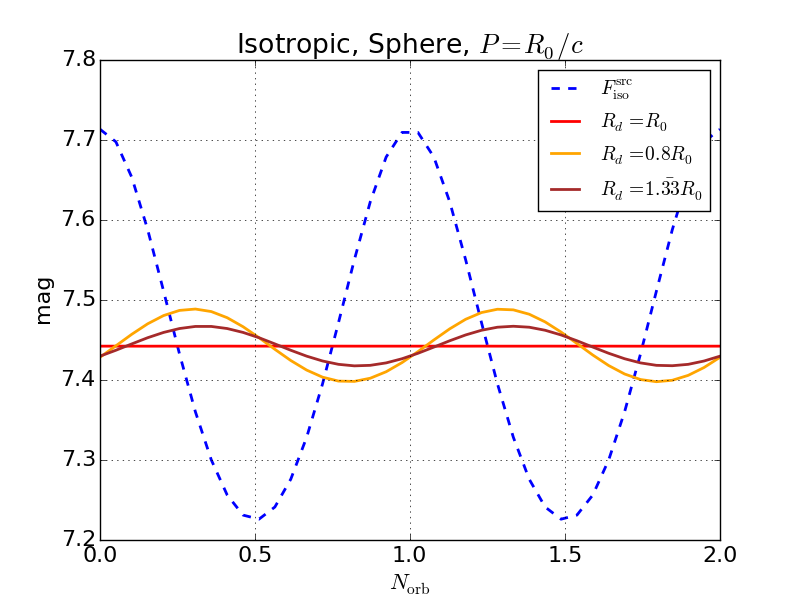
\includegraphics[scale=0.33]{figures/ch5/Sphere/FISO_Sphere_nrm0_Om1_VaryRin_numin0_numx5} & 
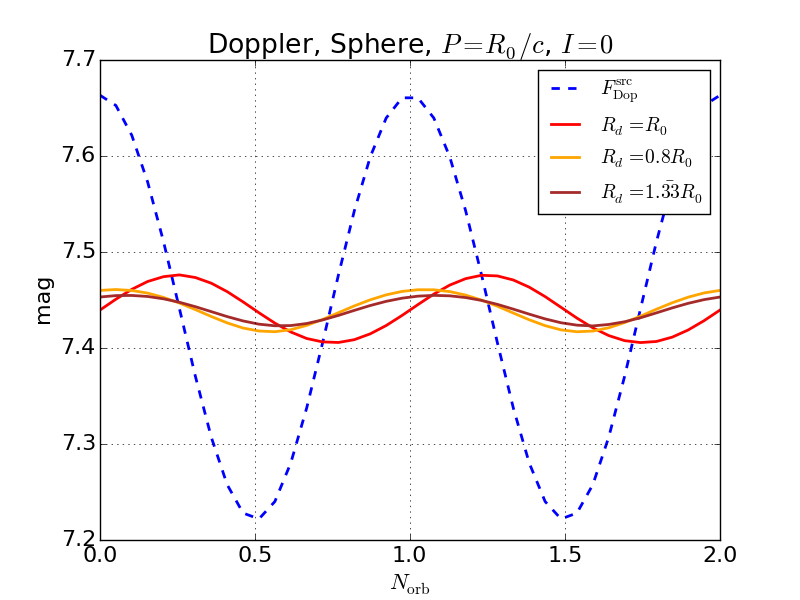
\includegraphics[scale=0.33]{figures/ch5/Sphere/FDop_R0_Sphere_nrm0__J0_Inc0_VaryRin_numin0_numx5} &
\end{array}$
\end{center}
\caption{Spherical dust shell model. The solid lines are the IR light curves
generated by reverberation of the UV/optical continuum (dashed blue line)
from a spherical dust shell with radius $R_d$ (measured in units of $R_0$ see
Table \ref{Table:params} for fiducial parameter values). The left panel is for
an isotropic central source, and the right panel is for a Doppler-boosted
central source.}
\label{Fig:SphDopvISO}
\end{figure}
%%%%%%%%%%%%%%%%%%%%%%%%%%%%%%%%%%%%%%%%%%%%%%%%







Finally we demonstrate the dependence of binary inclination angle in the
Doppler case. As discussed above, the observed IR amplitude in the Doppler
case drops to zero if there is no time variation in dust temperature in the
direction along the line of sight of the dust sphere. As illustrated in Figure
\ref{Fig:Sph_VarI}, this occurs when the binary is at a face-on inclination to
the observer line of sight. Because the fraction of dust temperature variation
along the line-of-sight is dependent only on the binary inclination in the
spherical case, IR and UV/optical amplitudes scale together, so that the
$A_{\rm IR}/A$ curve in Figure \ref{Fig:AIRoAUV_sp} is independent of binary
inclination. This scaling holds whenever the dust has back to front symmetry
along the line of sight, this can bee seen in Eq. (\ref{Eq:DopAIR_sp}) and in
the more general form, Eq. (\ref{Eq:AIR_thT}) below, where $\beta \cos{I}$
cancels in $A^{\rm{Dop}}_{\rm IR}/(\beta \cos{I})$. This will not be the case
for a \textit{misaligned} torus dust geometry.

%%%%%%%%%%%%%%%%%%%%%%%%%%%%%%%%%%%%%%%%%%%%%%%%
%%% FIGURE: Sphere IR light curves ISO vs Dop%%%
%%%%%%%%%%%%%%%%%%%%%%%%%%%%%%%%%%%%%%%%%%%%%%%%
\begin{figure}
\begin{center}
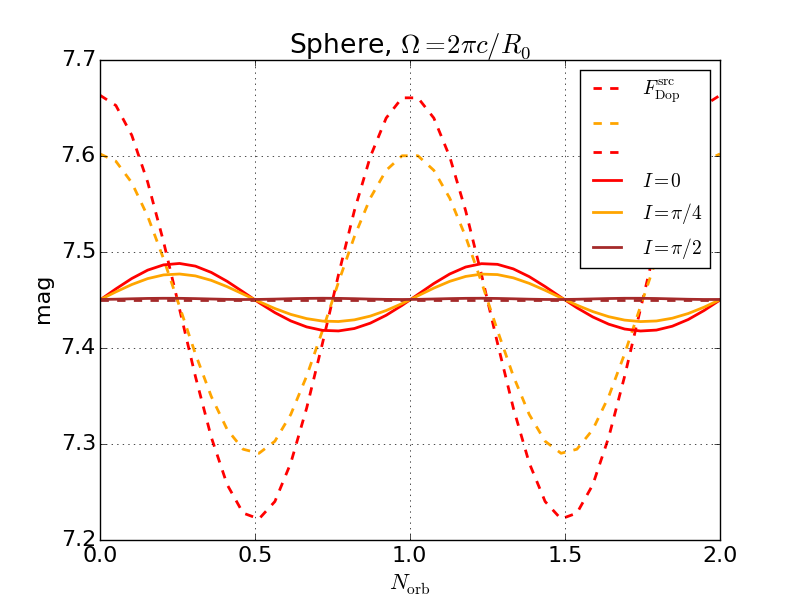
\includegraphics[scale=0.33]{figures/ch5/Sphere/FDop_Sphere_nrm0p0105326_Rde2p73218e+18_VaryInc_numin0_numx5} 
\end{center}
\caption{The same as Figure \ref{Fig:SphDopvISO} but for multiple binary 
inclination angles and $R_d = R_0$.}
\label{Fig:Sph_VarI}
\end{figure}
%%%%%%%%%%%%%%%%%%%%%%%%%%%%%%%%%%%%%%%%%%%%%%%%






 
\subsection{Geometrically-thin torus} 
\label{S:Interp:ThinTor}

The result from the previous section can be extended to a torus geometry with
infinitesimal radial extent, \textit{i.e.}, where regions of the sphere with
$\theta \leq \theta_T$ are removed. When the observer is looking down the axis
of the torus ($J=\pi/2$: see Figure \ref{Fig:Schm}), we find,
\begin{eqnarray}
L^{\rm{Iso}}_{\rm{IR}} &=&  \Sigma_d \pi  a^2_{\eff} L^0  \cos{\theta_T} \left[ 
  1 +  A  \ \rm{sinc}{\left( \Omega t_d \cos{\theta_T}\right)}  \sin{ \left( \Omega \left( t - t_d \right) \right)  }
   \right] \nonumber \\
   %
L^{\rm{Dop}}_{\rm{IR}} &=&  \Sigma_d \pi  a^2_{\eff} L^0 \cos{\theta_T} \left[ 
  1 +  \beta \cos{I}  \left[ \frac{    \rm{sinc}{ \left( \Omega t_d  \cos{\theta_T} \right)  }    }{\Omega t_d} 
  -  \frac{\cos{ \left(\Omega t_d  \cos{\theta_T} \right)}}{\Omega t_d }  \right] \cos{\left( \Omega \left( t - t_d \right) \right)}
   \right] ,
   \label{Eq:LIR_thT}
\end{eqnarray}
the relative amplitudes are 
\begin{eqnarray}
\frac{\Delta L^{\rm{Iso}}_{IR}/(L^0 \cos{\theta_T})}{\Delta L /L^0} \equiv \frac{A^{\rm{Iso}}_{\rm{IR}}}{A} &=&  \rm{sinc}{\left( 2 \pi \frac{t_d}{P} \cos{\theta_T} \right)}  \nonumber \\
   %
\frac{\Delta L^{\rm{Dop}}_{IR}/(L^0 \cos{\theta_T})}{\Delta L /L^0} \equiv \frac{A^{\rm{Dop}}_{\rm{IR}}}{\beta \cos{I}}  &=&  \frac{ \rm{sinc}{ \left( 2 \pi \frac{t_d}{P} \cos{\theta_T} \right)  }    }{2 \pi \frac{t_d}{P}} -  \frac{ \cos{ \left(2 \pi \frac{t_d}{P} \cos{\theta_T} \right) } }{ 2 \pi \frac{t_d}{P} },
   \label{Eq:AIR_thT}
\end{eqnarray}
and because the dust distribution is centered around the source, the phase
lags are given identically to the spherical case (Eqs. \ref{Eq:ISOLags} and
\ref{Eq:DOPLags}).






Figure \ref{Fig:AIRoAUV_tr} explores the torus solutions. The first panel in
Figure \ref{Fig:AIRoAUV_tr} plots the relative IR to UV/optical variability
amplitudes for different opening angles, for an observer looking down the axis
of the opening. The analytic result Eq. (\ref{Eq:LIR_thT}) (solid lines in
Figure \ref{Fig:AIRoAUV_tr}) matches the result of the corresponding numerical
evaluation of the calculation presented in \S \ref{S:Derivation} (x's in
Figure \ref{Fig:AIRoAUV_tr}). The middle and right panels of Figure
\ref{Fig:AIRoAUV_tr} extend upon the analytic result by rotating the torus by
angles $J=\pi/4$ and $J=0$.

The effect of increasing the torus opening angle $\theta_T$ is two fold, it
decreases the total IR luminosity, not reflected in the relative amplitude of
variability but important for the size of absolute luminosity variations. It
also moves the location of the zeros of the IR amplitude curve to larger
$t_d/P$. Recalling the discussion in the previous section, the IR amplitude is
nullified, in the isotropic case, when an integer number of variability
periods matches the light crossing time of the line-of-sight dust structure.
Depending on the orientation $J$ of the torus, $\theta_T$ changes this line of
sight extent, and hence the zero amplitude values of $t_d/P$.

 

When looking down the opening of the torus ($J=\pi/2$), a non-zero opening
angle decreases the line-of-sight extent of the dust shell from $2 R_d$ in the
spherical case to $2 R_d\cos{\theta_T}$ (this can be discerned from Eq.
(\ref{Eq:LIR_thT}) and visualized with Figure \ref{Fig:Schm}). As the torus is
tilted away from $J=\pi/2$, the relationship between the closest and furthest
points of the sphere becomes less dependent on $\theta_T$. To bracket the
dependence on $\theta_T$ and $J$ we consider the extreme cases of a face-on
and edge-on dust rings.

Because $\rm{sinc}{(0)}\rightarrow 1$, Eq. (\ref{Eq:AIRoAUV}) tells us that
the limit of a face-on ring ($\theta_T \rightarrow \pi/2$, $J=\pi/2$),
recovers the UV/optical amplitude but at lower IR luminosity set by the
covering factor of the thin ring. This is simply because time delay effects
are no longer important for a face-on ring. Graphically, this is exhibited in
the left panel of Figure \ref{Fig:AIRoAUV_tr}; for larger $\theta_T$ the
$A_{\rm{IR}}/A$ curves stretch out further to the right at the expense of
lower IR luminosity. Hence for a $J=\pi/2$ torus the limiting behavior is set
by the black curve for a dust sphere and a line at $A_{\rm{IR}}/A=1$ for a
face on (zero-luminosity) dust ring.

In the limit of a thin, edge-on ring ($\theta_T \rightarrow \pi/2 -
\tan^{-1}{(a_{\rm{eff}}/R_d)}$, $J=0$) the solution for reverberated emission
becomes
\begin{equation}
L^{\rm{Iso}}_{\rm{IR}} =  \Sigma_d \pi  a^2_{\eff} \frac{ a_{\rm{eff}} }{ R_d } L^0  \left[ 1 +  A  \ J_0\left( \Omega t_d \right)  \sin{ \left( \Omega \left( t - t_d \right) \right)  } 
   \right] \quad \rm{Edge-On-Ring}
   \label{Eq:ISO_Ring}
\end{equation}
where $J_0(z)$ is the zeroth order Bessel function of the first kind and the
solution is valid for $a_{\rm{eff}} \ll R_d$. This solution is plotted in the
right $J=0$ panel of Figure \ref{Fig:AIRoAUV_tr} and shows that, for a $J=0$
torus, the possible amplitudes are bracketed by the two analytic solutions for
a sphere and a face-on ring. By the above reasoning, the $J=0$ and $J=\pi/2$
panels in Figure \ref{Fig:AIRoAUV_tr} show the limiting behaviors of the IR
variability amplitude, from an isotropic source, over the range of possible
torus inclinations and opening angles.




%%%%%%%%%%%%%%%%%%%%%%%%%%%%%%%%%%%%%%%%%%%%%%%%
%%% FIGURE: AIR/A ISO %%%
%%%%%%%%%%%%%%%%%%%%%%%%%%%%%%%%%%%%%%%%%%%%%%%%
\begin{figure}
\begin{center}$
\begin{array}{c c c}
%FISO and DOP 
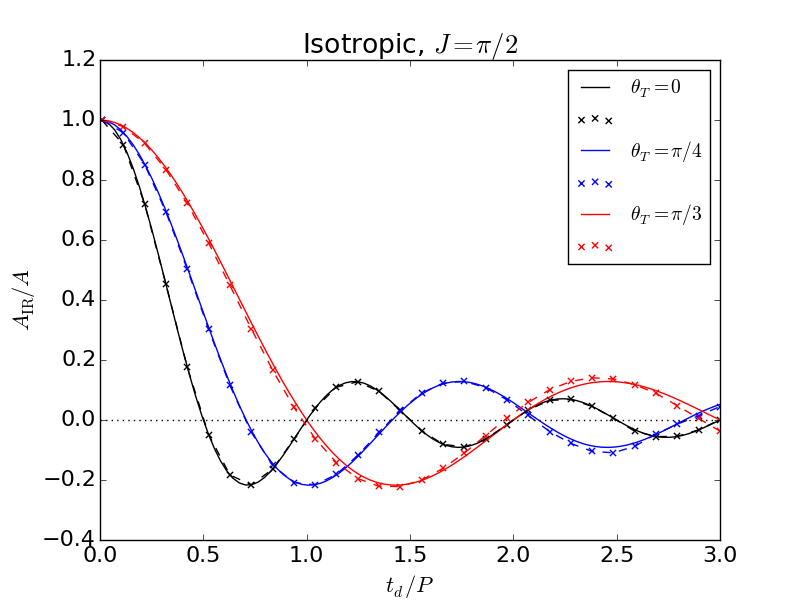
\includegraphics[scale=0.27]{figures/ch5/AIRplots/AIRoAUV_REL_J1p5708_numin0_numx3.png} & 
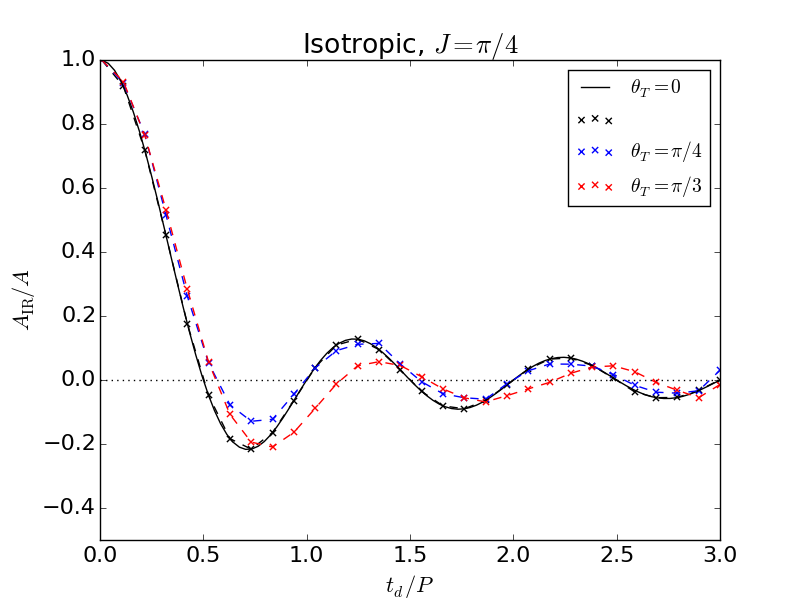
\includegraphics[scale=0.27]{figures/ch5/AIRplots/AIRoAUV_REL_J0p785398_numin0_numx3.png} &
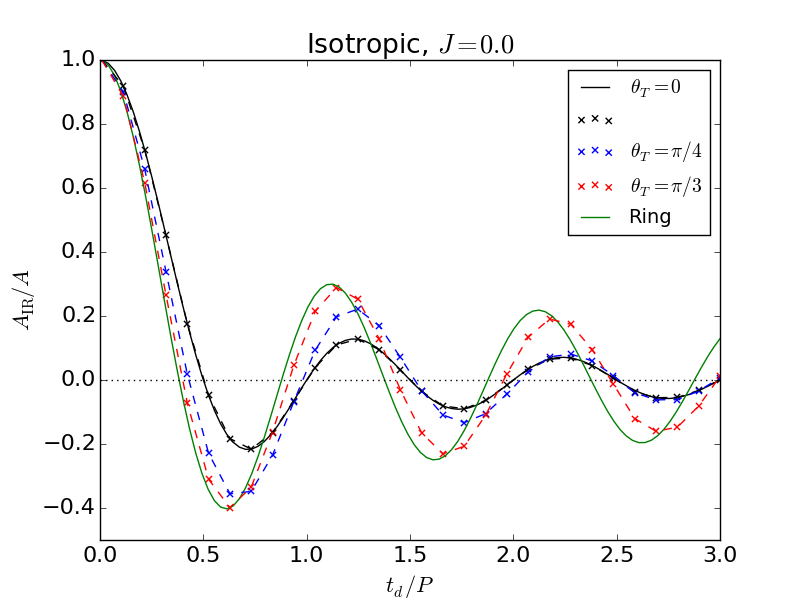
\includegraphics[scale=0.27]{figures/ch5/AIRplots/AIRoAUV_REL_J0_numin0_numx3.png} 
\end{array}$
\end{center}
\caption{
The amplitude of IR variability  relative to the UV/optical amplitude,
$A_{\rm{IR}}/A$, for a radially thin, dust torus which absorbs all incident
UV/optical radiation and emits it in IR. Each panel varies the opening angle
$\theta_T$ of the dust torus for a different torus inclination angle $J$. The
solid lines are the analytic solutions Eq. (\ref{Eq:LIR_thT}) in the limit
that $J=\pi/2$. The green line in the right panel is the analytic solution Eq.
(\ref{Eq:ISO_Ring}) for a face-on ring of dust ($J=0$, $\theta_T = \pi/2$).
The x's are the result of numerical calculations presented in \S
\ref{S:Derivation}.
} 
\label{Fig:AIRoAUV_tr}
\end{figure}
%%%%%%%%%%%%%%%%%%%%%%%%%%%%%%%%%%%%%%%%%%%%%%%%


Figure \ref{Fig:AIRoAUVDop_tr} explores the dependence of IR variability
amplitude on dust geometry for the Doppler source with an edge-on binary
inclination. The behaviour is similar to that of the isotropic case, with the
$J=0$ and $J=\pi/2$ sphere and ring cases bracketing the possible behavior.



We first consider the limiting cases of a face-on and an edge-on dust ring for
the Doppler-boosted source. For a face-on dust ring ($J=\pi/2$), and any
binary inclination, the amplitude of variability for Doppler-boosted sources
drops to zero because the dust has no extent along the line of sight, and
hence no time delay structure.

The edge-on dust ring exhibits reverberated IR luminosity
\begin{equation}
L^{\rm{Dop}}_{\rm{IR}} =  \Sigma_d \pi  a^2_{\eff}  \frac{ a_{\rm{eff}} }{ R_d } L^0   \left[ 1 +  \beta \cos{I}  \ J_1\left( \Omega t_d \right)  \cos{ \left( \Omega \left( t - t_d \right) \right)  } 
   \right] \quad \rm{Edge-On-Ring}
   \label{Eq:DOP_Ring}
\end{equation}
where $J_1(z)$ is the first order Bessel function of the first
kind.\footnote{Note again that the derivate of $A^{\rm{Iso}}_{\rm{IR}}$, with
respect to $t_d/P$, is $-A^{\rm{Dop}}_{\rm{IR}}$.} This solution is plotted in
the right $J=0$ panel of Figure \ref{Fig:AIRoAUVDop_tr}.





%%%%%%%%%%%%%%%%%%%%%%%%%%%%%%%%%%%%%%%%%%%%%%%%
%%% FIGURE: AIR/A Torus 1 DOP%%%
%%%%%%%%%%%%%%%%%%%%%%%%%%%%%%%%%%%%%%%%%%%%%%%%
\begin{figure}
\begin{center}$
\begin{array}{c c c}
%FISO and DOP 
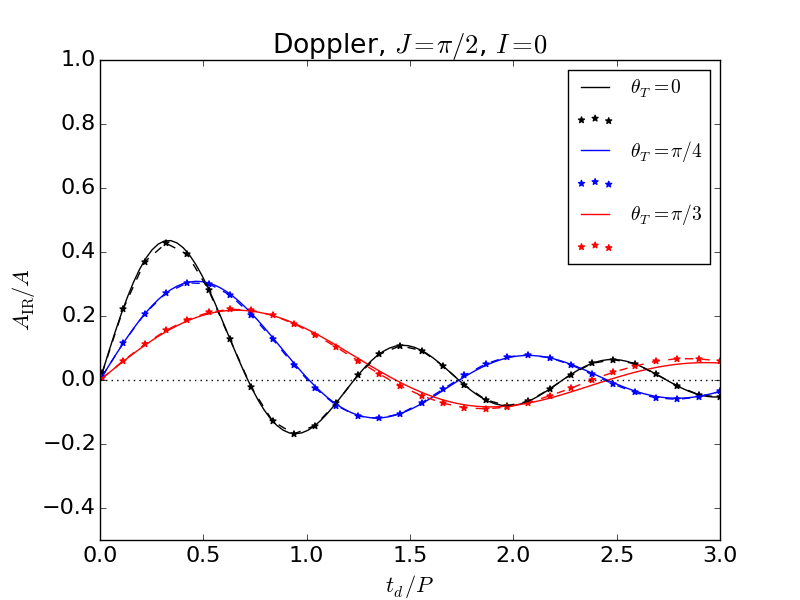
\includegraphics[scale=0.27]{figures/ch5/AIRplots/AIRoAUVDop_REL_J1p5708_numin0_numx3.png} &
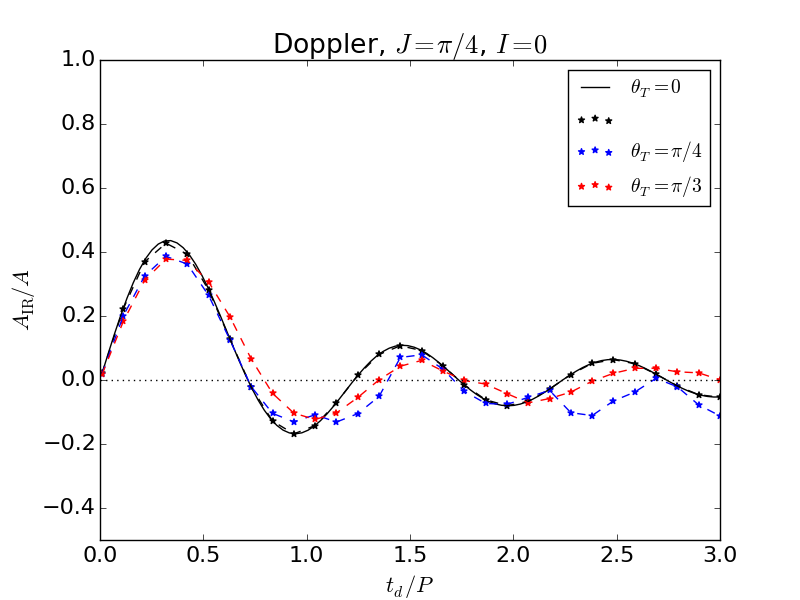
\includegraphics[scale=0.27]{figures/ch5/AIRplots/AIRoAUVDop_REL_J0p785398_numin0_numx3} &
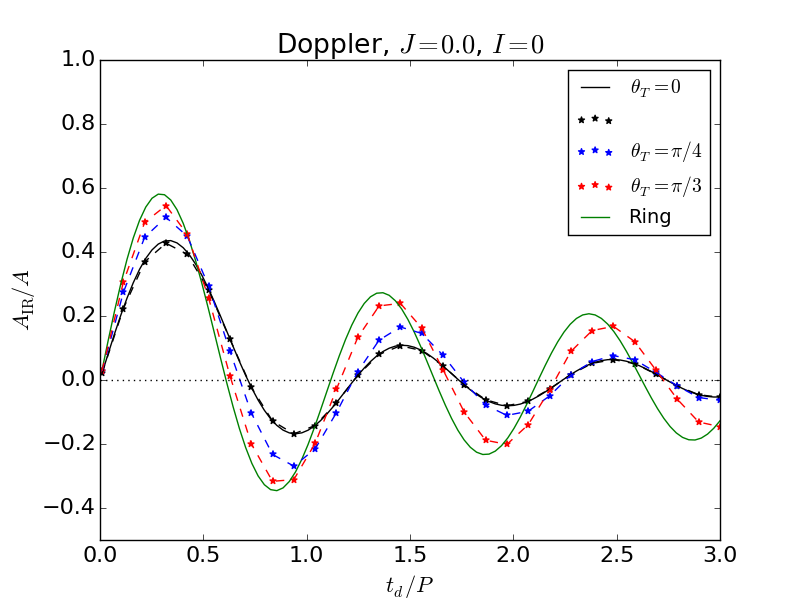
\includegraphics[scale=0.27]{figures/ch5/AIRplots/AIRoAUVDop_REL_J0_numin0_numx3} 
\end{array}$
\end{center}
%
\caption{The same as Figure \ref{Fig:AIRoAUV_tr}, but for the Doppler-boosted source with edge-on
binary inclination. Solid lines plot analytic solutions when available.} 
%
\label{Fig:AIRoAUVDop_tr}
\end{figure}
%%%%%%%%%%%%%%%%%%%%%%%%%%%%%%%%%%%%%%%%%%%%%%%%









In Figure \ref{Fig:ShTor_DopvISO} we plot the IR (solid lines) and optical
light-curves (dashed lines) for various torus opening and inclination angles,
choosing a value of $t_d/P=0.6$. We recover the amplitudes of Figure
\ref{Fig:AIRoAUV_tr} and \ref{Fig:AIRoAUVDop_tr} and observe the expected
dimming of the IR light curves for larger torus opening angles. In both the
isotropic and Doppler cases, the phase lag of the IR to the UV/optical is
independent of the dust geometry parameters $J$ and $\theta_T$. In the
isotropic cases (left panels of Figure \ref{Fig:ShTor_DopvISO}) the one half
cycle phase shift between the $J=\pi/2$ and $J=0$ curves is consistent with
the corresponding signs of $A_{\rm{IR}}/A$ in Figure \ref{Fig:AIRoAUV_tr}; For
$J=\pi/2$, $A_{\rm{IR}}/A <0$ for the chosen $\theta_T$, while for $J=0$,
$A_{\rm{IR}}/A > 0$. See the previous section for a discussion of this phase
shift.





%%%%%%%%%%%%%%%%%%%%%%%%%%%%%%%%%%%%%%%%%%%%%%%%
%%% FIGURE: Sphere IR light curves ISO vs Dop%%%
%%%%%%%%%%%%%%%%%%%%%%%%%%%%%%%%%%%%%%%%%%%%%%%%
\begin{figure}
\begin{center}$
\begin{array}{c c}
%FISO and DOP  vary Rin
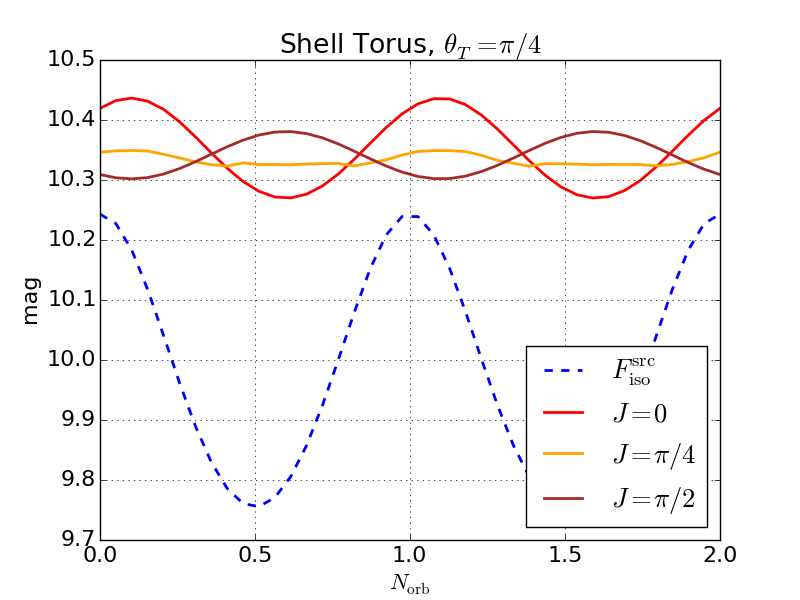
\includegraphics[scale=0.33]{figures/ch5/ShTor_Thin/FISO_ShTor_Thin_nrm0__Rin2p73218e+18_Inc0_thetaT0p785398_VaryJ_numin0_numx6} & 
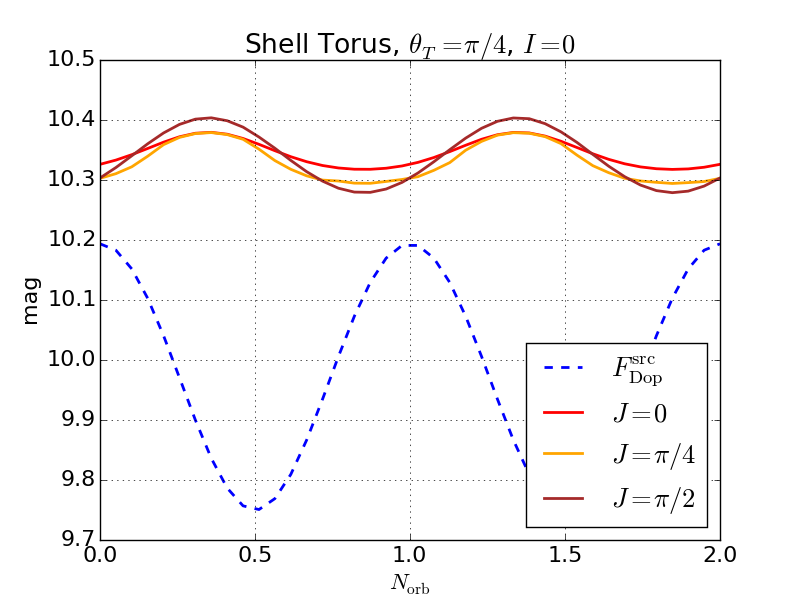
\includegraphics[scale=0.33]{figures/ch5/ShTor_Thin/FDop_ShTor_Thin_nrm0__Rin2p73218e+18_Inc0_thetaT0p785398_VaryJ_numin0_numx6} \\
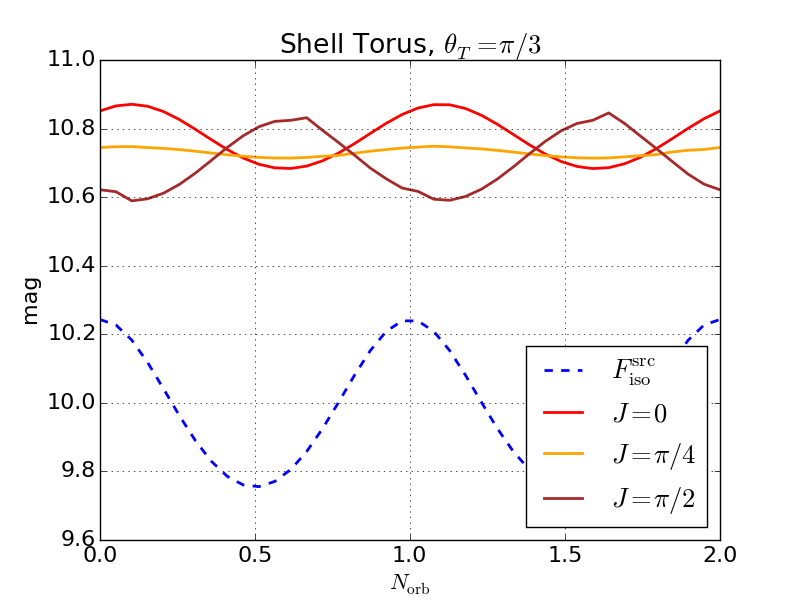
\includegraphics[scale=0.33]{figures/ch5/ShTor_Thin/FISO_ShTor_Thin_nrm0__Rin2p73218e+18_Inc0_thetaT1p0472_VaryJ_numin0_numx6} &
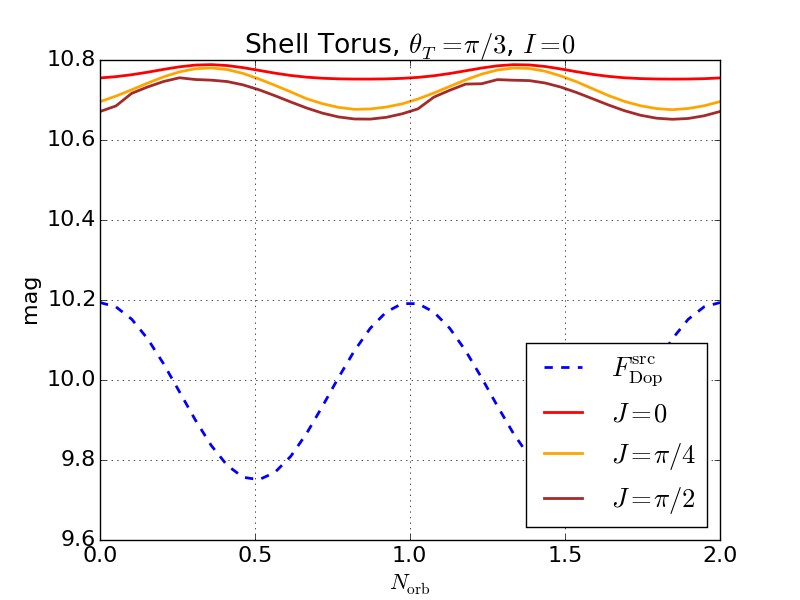
\includegraphics[scale=0.33]{figures/ch5/ShTor_Thin/FDop_ShTor_Thin_nrm0__Rin2p73218e+18_Inc0_thetaT1p0472_VaryJ_numin0_numx6}
\end{array}$
\end{center}
%
\caption{The same as Figure \ref{Fig:SphDopvISO} but for the torus dust shell
model. Here $R_d = 0.6 R_0$, each panel plots IR light curves for different
torus inclination angles, and for a chosen torus opening angle $\theta_T$. The
left panel assumes an isotropic central source while the right panels assume a
Doppler-boosted source.}
%
\label{Fig:ShTor_DopvISO}
\end{figure}
%%%%%%%%%%%%%%%%%%%%%%%%%%%%%%%%%%%%%%%%%%%%%%%%



Finally, we explore the effects of binary inclination in the torus dust model.
With the freedom to orient the binary plane relative to a non-spherical dust
structure through parameters $I$ and $J$ (for $\theta_T \neq 0$), the
possibility of generating IR variability with no observed UV/optical variability
arises. Figure \ref{Fig:ShTor_VarI} demonstrates that when the binary is
face on, there is no observed UV/optical variability (\textit{e.g.} Eq.
(\ref{Eq:vlos})), but IR variability still persists. 

For the spherical model, a face-on binary generates no IR variability because
there is no time changing emission between the front and back hemispheres of
the dust shell, the integrated dust emission is constant. This back-to-front
symmetry is broken in the case of a torus dust shell, as long as the dust is
not symmetric around the plane perpendicular to the observer that contains
the source, \textit{i.e.}, $\theta_T \neq 0$, $J\neq 0$ and $J\neq \pi/2$.




%%%%%%%%%%%%%%%%%%%%%%%%%%%%%%%%%%%%%%%%%%%%%%%%
%%% FIGURE: Sphere IR light curves ISO vs Dop%%%
%%%%%%%%%%%%%%%%%%%%%%%%%%%%%%%%%%%%%%%%%%%%%%%%
\begin{figure}
\begin{center}
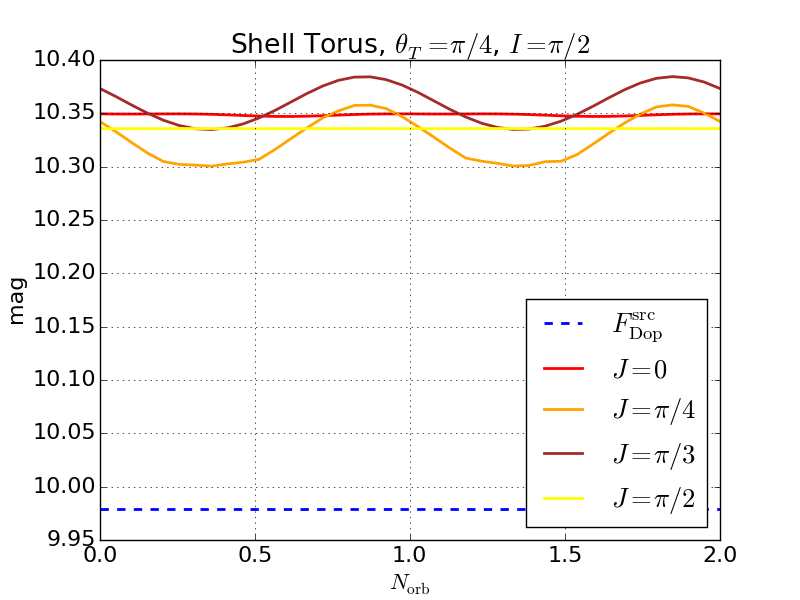
\includegraphics[scale=0.33]{figures/ch5/ShTor_Thin/FDop_ShTor_Thin_nrm0__Rin2p73218e+18_Inc1p5708_thetaT0p785398_VaryJ_numin0_numx6} 
\end{center}
%
\caption{The same as Figure \ref{Fig:ShTor_DopvISO} but for a face-on binary
inclination. For all but extreme torus inclinations $J=0, \pi/2$,
significant IR variability persists even when no UV/optical variability is
observed.}
%
\label{Fig:ShTor_VarI}
\end{figure}
%%%%%%%%%%%%%%%%%%%%%%%%%%%%%%%%%%%%%%%%%%%%%%%%


























%%%%%CUT OUT PG 1302 STUFF FOR THESIS








% \section{Application to MBHB candidate PG 1302}
% \label{S:PG1302}
% We now apply our models to the periodically variable quasar and MBHB candidate
% PG 1302-102. We use data published by J15 from the W1 and W2 band of the WISE
% instrument at $3.4 \mu$m ($2.8 \rightarrow 4.0 \mu$m) and $4.6 \mu$m ($3.9
% \rightarrow 5.3 \mu$m) respectively. The longer wavelength WISE W3 ($12 \mu$m)
% and W4 ($22 \mu$m) bands are not reported because these bands only took data
% during the cryogenic phase of the WISE mission (before it ran out of coolant
% circa late 2010) and the data is too sparse to be useful for period recovery
% (see J15)\footnote{The W3 and W4 data, even if only at one epoch, would be
% useful constraints on PG 1302's SED. \textcolor{red}{Waiting on this data}}.
% Data for W1 and W2, however, exists at six month intervals from 2010 to July
% 2015 with a three year gap during hibernation between 2011 and 2014. Each
% epoch of WISE measurements consists of $\sim 10$ data points taken within a few
% days of each other. To fit models to the WISE data, we use a single data point
% at each epoch with mean and variance given by the average mean and variance at
% that epoch (see Figure \ref{Fig:PGBestFits}).




% \subsection{Strategy}
% From our models we aim to determine whether the IR data from PG 1302 is
% consistent with reverberation from a periodic UV/optical source, and whether
% such a source is varying isotropically, or via the Doppler-boost mechanism. We
% also constrain the parameters of a putative dust torus.


% Given the period $P$ of source variability, the primary observables are the
% relative amplitude and phase of the IR light curves. We have shown that the
% relative amplitude of IR variability $A_{\rm{IR}}/A$ is dependent on the ratio
% $t_d/P$, the opening angle of the dust torus $\theta_T$ (the covering factor),
% and the torus inclination to the line of sight $J$; the IR phase lag
% $\Phi$ is dependent on the ratio $t_d/P$. For a Doppler-boosted source the IR
% amplitude also depends on binary inclination angle $I$ and source spectral
% slope $\alpha_{\nu}$.

% We measure $P$, $\Phi$ and $A_{\rm{IR}}/A$ directly from the optical and WISE
% light curves. A blackbody spectral fit to the WISE data allows measurement of
% the total IR luminosity and also the fraction of total luminosity in the IR.
% Together these determine the dust covering factor $\cos{\theta_T}$ and the
% dust radius $R_d$, yielding $\theta_T$ and $t_d/P$. The phase lag $\Phi$
% provides a second measurement of $t_d/P$. Hence we may use the inferred values
% of $t_d/P$ and $\theta_T$ and determine values of $J$ that yield the measured
% value of $A_{\rm{IR}}/A$, if they exist. In the Doppler case we may measure
% $\alpha_{\nu}$ and choose the binary orbital speed and inclination based on
% fits to the optical data \citep[\textit{e.g.}][]{PG1302Nature:2015b}. With
% knowledge of the binary period, a consistent model yields constraints on the
% dust torus opening angle, inclination, and radius, as well as the binary
% inclination for a Doppler-boosted source.

% Once we have narrowed down the available parameter space for PG 1302, we
% perform fits of our models to the optical, W1 and W2 data, numerically
% calculating Eq. (\ref{Eq:FISO}) over the W1 and W2 frequency ranges.






% \subsection{Measurements}
% To extract the phase lag and relative amplitude of IR light curves, we fit
% separate sinusoids to the V-band, W1, and W2 data. For all model fitting we
% minimize a simple $\chi^2$ likelihood using the Markov Chain Monte Carlo
% algorithms in the publicly available code \textsc{emcee} \citep{DFM:2013}.
% Details are found in the Appendix.

% Fixing the observed period of PG 1302 to $P=1884$ days, we fit sinusoids of
% the form $\mathcal{A} \sin{\Omega\left(t-t_0\right)} + \mathcal{B}$. The best
% fit sinusoid parameters are recorded in Table \ref{Table:SinParams}.





% \begin{table}
% \begin{center}
% \begin{tabular}{ c | c | c | c }
% %
% Model: &    $\mathcal{A} \sin{\Omega\left(t-t_0\right)} + \mathcal{B}$ &   $\Omega = 2\pi/1884$ day$^{-1}$ & \\
% \hline
%                         & V                    & W1                    &  W2                   \\
% \hline
% $\mathcal{A}$ [mag]     & $0.1269^{+0.0004}_{-0.0004}$ & $0.0862^{+0.0158}_{-0.0271}$ &  $0.0813^{+0.0157}_{-0.0260}$    \\ \\
% $t_0$ [days]            & $1403.4^{+0.7}_{-0.8}$    & $346.7^{+24.6}_{-37.3}$      &  $399.9^{+23.1}_{-55.0}$ \\ \\
% $\mathcal{B}$ [mag]     & $14.8329^{+0.0003}_{-0.0003}$ & $11.39^{+0.01}_{-0.02}$      &  $10.31^{+0.01}_{-0.02}$  \\  \\
% $\chi^2_{\rm{red}}$     & 40.5                 & 2.0                  & 0.4      
% %
%  \end{tabular}
% \caption{Best fit sinusoid parameters. The reduced $\chi^2$ statistic is smaller for the W1 and W2 data because we have binned each epoch into one data point as explained in the Appendix.}
% \end{center}
% \label{Table:SinParams}
% \end{table}




% The best fit sinusoid amplitudes in Table \ref{Table:SinParams} give relative 
% IR to optical amplitudes
% \begin{eqnarray}  \nonumber
% \frac{A_{\rm{W1}}}{A_{\rm{V}}}  &\approx& 0.68^{+0.12}_{-0.21} \\
% \frac{A_{\rm{W2}}}{A_{\rm{V}}}  &\approx& 0.64^{+0.12}_{-0.20} \nonumber
% \end{eqnarray}
% To compare to the analytic solutions we require the quantity $A_{\rm{IR}}/A$,
% however, we face an incomplete knowledge of the frequency dependence of source
% variability. Thus far we have assumed that the amplitude of source variability
% $A$ is given by
% \begin{equation}  
% A = \frac{\int^{\infty}_{0}{L^0_{\nu} A(\nu)  d \nu} }{ \int^{\infty}_{0}{L^0_{\nu}} d \nu }, 
% \end{equation}
% where $A(\nu)$ is the frequency dependent amplitude of source variability. The
% measured quantities of $A$ (\textit{e.g.} the V band value above) are given
% by the above equation but integrated over the relevant observational band. We
% have three measurements of $A$, the extremes of which are $A_{\rm{V}} \sim 0.14$ mag
% and $A_{\rm{FUV}} \sim 0.37$ mag \citep{PG1302Nature:2015b}. To compare to our
% model we must translate this limited knowledge of $A(\nu)$ into an estimate
% for $A$. Here we simply assume that the known values, given by
% the V-band and the FUV amplitudes, bracket the actual value. In the Doppler-
% boost case, this is a reasonable assumption as the UV and optical portions of
% the PG 1302 spectrum bracket the range of spectral slopes and occur on
% opposing sides of the peak of $\lambda F_{\lambda}$ \citep{Graham+2015a}.
% Choosing the same approach for the frequency dependence of the IR emission we
% find the range of possible relative amplitudes
% $A_{\rm{IR}}/A_{\rm{V}}$
% \begin{eqnarray} \nonumber
% \frac{A_{\rm{IR}}}{A_{\rm{V}}} =  \frac{A_{\rm{W2}}}{A_{\rm{FUV}}} \rightarrow \frac{A_{\rm{W1}}}{A_{\rm{V}}} &\approx& 0.17  \rightarrow 0.8 .
% \end{eqnarray}




% The best fit phase lags measured relative to the V band give
% \begin{eqnarray} 
% \Phi_{W1} &\approx& (0.284+m)^{+0.017}_{-0.026} \nonumber \\
% \Phi_{W2} &\approx& (0.319+m)^{+0.016}_{-0.038} \quad m=0,1,2...\nonumber
% \end{eqnarray}
% Using the phase lags and uncertainties measured in J15, we find
% \begin{eqnarray} 
% \Phi_{W1} &\approx& 0.18 \pm 0.08 + m \nonumber \\
% \Phi_{W2} &\approx& 0.28 \pm 0.08 + m \quad m=0,1,2... \nonumber
% \end{eqnarray}
% from which values of $t_d/P$ are derived from Eq. (\ref{Eq:ISOLags}) and
% (\ref{Eq:DOPLags}) for both the isotropic and Doppler cases. Our values of 
% the phase lag are consistent with those of J15, though our upper limit on the 
% W1 phase lag extends out of the range found by J15. We use the range spanned 
% by both measurements to be conservative.





% To place further constraints on $t_d/P$, and to constrain the covering
% fraction of the dust torus $\theta_T$, we estimate the fractional and total
% luminosity in IR emitted by PG 1302. We find the best fit area and temperature
% of a torus shell which emits as a blackbody (setting the emission efficiency
% $Q_{\nu}= 1$).\footnote{The result does not greatly differ if we fit for the
% efficiency parameters $\nu_0$ and $k$ (see Table \ref{Table:params}).} We
% integrate the best fit blackbody spectrum over all frequencies to estimate the
% total IR luminosity. Given the flux in each WISE band, $F_{\rm{W1}} = 8.83 \pm
% 0.18$ mJy and $F_{\rm{W2}} = 13.33 \pm 0.26$ mJy (one-$\sigma$ errors), we
% find a blackbody with best fit dust temperature $T = 880.6 \pm 14.2$K and with
% opening angle and radius given by $R_d \sqrt{\cos{\theta_T}} = 1.48 \pm 0.05$
% pc. Errors are quoted as the average of lower and upper $15^{\rm{th}}$
% percentile values (see the Appendix for details). Integrating, we find
% \begin{equation}
% \frac{ L_{\rm{IR}} }{ L_{\rm{tot}} } \approx 0.13 \pm 0.06,  \nonumber
% \end{equation}
% where $L_{\rm{tot}} \approx 6.78 \pm 2.71 \times 10^{46}$ is derived from the
% V-band luminosity and a bolometric correction of 10
% \citep[\textit{e.g.}][]{PG1302Nature:2015b}, the error estimate for
% $L_{\rm{tot}}$ is based on adopting bolometric corrections of $10\pm4$. The
% error estimate for ${ L_{\rm{IR}} }/{ L_{\rm{tot}} }$ is derived from the
% error on $L_{\rm{tot}}$ and from propagating the quoted errors on the
% parameters from the blackbody fit into the calculation of $L_{\rm{IR}}$. There
% is also a, not included, systematic uncertainty due to the choice of fitting a
% blackbody to the data.

% %DD:
% \textcolor{red}{Bolometric Correction of $10 \pm 4$ should be backed up} \\
% \textcolor{red}{Waiting on W3 and W4 values from Hyunsung - results may change with these included}


% The ratio of the IR to UV/optical luminosity gives the covering factor $f$ of
% the torus and hence the opening angle of the dust torus, $f \equiv
% L_{\rm{IR}}/L_{\rm{tot}} = \cos{\theta_T}$. From the above condition on the
% area of the emitting region ($4 \pi R^2_d \cos{\theta_T}$) and the measurement
% of $\cos{\theta_T}$, we require the radius of a torus shell with opening angle
% $\cos{\theta_T} = 0.13 \pm 0.06$ to be $R_d = 4.1 \pm 0.9$ pc which gives a
% value of $t_d/P = 3.3 \pm 0.7$ for PG 1302.

% For consistency we further require that the dust have the temperature of the
% best fit blackbody at the best fit radius. This, however, is not the case, the
% best fit temperature implies that the dust lies at a radius $2.0 \pm 0.4$ pc
% with uncertainty due to the uncertainty in bolometric luminosity and the
% uncertainty in $T_d$.  This discrepancy suggests that one of the following
% assumptions must break down:
% \begin{enumerate}
% \item The dust does not emit as a pure blackbody and hence the integrated IR luminosity which fixes the best-fit radius of the dust sphere is biased.  
% \item The dust absorption/emission frequency is more complicated than the simple power law employed here, yielding different equilibrium dust temperatures (\textit{i.e.} this discrepancy does not go away when fitting also for efficiency parameters $k$ and $\nu_0$).
% \item The dust is not optically thick to UV/optical or it is clumpy and hence can consistently exist at the best fit equilibrium temperature at a different radius.
% \end{enumerate}
% Assuming this discrepancy can be remedied, we use our derived values for the
% dust radius, covering factor, amplitude of modulation, and  phase lag to
% constrain model parameters for a dust torus surrounding PG 1302.




% %TABLE OF MEASURED/Inferred VALUES
% \begin{table}
% \begin{center}
% \begin{tabular}{ c | c | c | c }
% %
% Measured Quantity       &    Light Curve                            &   BlackBody Fit \\
% \hline
% $A_{\rm{IR}}/A$         &  $0.17 \rightarrow 0.80$                  &  --   \\
% $\Phi_{\rm{W1}}$        &  $0.10 \rightarrow 0.30$ cycles           &  -- \\
% $\Phi_{\rm{W2}}$        &  $0.20 \rightarrow 0.36$ cycles           &  -- \\
% $t_d/P$                 &  Eqs. \ref{Eq:ISOLags}, \ref{Eq:DOPLags}  & $3.3 \pm 0.7$   \\
% $\cos{\theta_T}$        &  --                                       & $0.13 \pm 0.06$    
% %
% \end{tabular}
% \caption{Measured quantities used to determine the nature of the IR light
% curves of PG 1302. The first column displays quantities found directly from
% fitting the IR and optical light curves. The second column displays quantities
% measured from fitting a blackbody spectrum to the average WISE band fluxes and
% inferring the radius and covering factor of the IR emitting torus.}
% \end{center}
% \label{Table:IRmeasures}
% \end{table}

% Table \ref{Table:IRmeasures} summarizes our measured values for the IR relevant PG 1302 quantities.

% \textcolor{red}{Latex insists on calling this Table 5.2 instead of Table 3 even though the hyperlink is to the correct table}


% \subsection{Findings}
% \subsubsection{Allowed parameter space}
% Informed by the quantities measured in the previous section (Table
% \ref{Table:IRmeasures}), Figure \ref{Fig:PGConts} plots the allowed regions of
% $\cos{\theta_T}$, $t_d/P$, and $A_{\rm{IR}}/A$ parameter space. The left
% column is for an isotropically varying source and the right column is for a
% Doppler-boosted source. The top row shades allowed regions of
% ($\cos{\theta_T}$, $t_d/P$) parameter space and the bottom row shades regions
% of ($A_{\rm{IR}}/A$, $t_d/P$) parameter space.

% In the top row of Figure \ref{Fig:PGConts} the blue regions show the allowed
% values of the covering factor, while the orange regions show the allowed
% values of the ratio $t_d/P$. The disjointed nature of the orange regions is
% from the ambiguity in adding an integer number of periods to the phase lag
% measurement and also from the half-cycle phase change occurring when
% $A_{\rm{IR}}/A$ changes sign (Eqs. (\ref{Eq:ISOLags}) and (\ref{Eq:DOPLags})).
% The solid orange region spanning the entire y-axis is from the measurement of
% $R_d$ in combination with $P$ taken from the blackbody fit to the average
% WISE-band fluxes. The models for the amplitude of variability are expressed by
% the red and green regions. The red regions show where the predicted IR
% amplitude falls within the measured value for a torus inclination angle of
% $J=\pi/2$ (looking down the opening- axis of the torus, Eqs.
% (\ref{Eq:LIR_thT})). The green regions are the same as the red regions but for
% an edge on dust ring (Eqs. (\ref{Eq:ISO_Ring}) and (\ref{Eq:DOP_Ring})). As
% the case of an edge-on ring and the $J=\pi/2$ torus bracket the range of
% possibilities for the IR amplitude, we conclude that a consistent model for
% periodically reverberated emission is realized only if blue, orange, and red
% \textit{or} blue, orange, and green regions overlap in Figure
% \ref{Fig:PGConts}.

% The bottom row shows the same restrictions on parameter space in the
% ($A_{\rm{IR}}/A$, $t_d/P$) plane and with $A_{\rm{IR}}/A$ curves drawn for
% specific choices of $\theta_T$ and for limiting torus inclination angles
% $J=\pi/2$ (red) and $J=0$ (green). We shade constraints from the W1 data
% yellow and constraints from the W2 data red. In the isotropic case, we draw a
% specific solution for which the measurements are consistent (dashed red line).

% %possible solutions
% We find two fully consistent solutions, both for an isotropically varying
% source. The largest part of parameter space favors an isotropic source
% surrounded by a nearly face-on ($J\sim \pi/2$) dust torus with a large opening
% angle $0.07 \lsim \cos{\theta_T} \lsim 0.15$, resembling a ring with radius
% $R_d \sim 4.1 \pm 0.9$ pc ($2.7 \lsim t_d/P \lsim 4$), or the inner edge of a
% disc with aspect ratio given by $\cos{\theta_T}$ and the same inner-radius.
% The second solution is for an isotropic source surrounded by an \textit{edge-
% on} disc with the same opening angle and an inner radius of $\sim 3.8$ pc.

% The reason for face-on ring solution is the large relative IR amplitudes required by
% the data. Such amplitudes can only be reached when light travel time becomes
% less important and the IR variability amplitude approaches the UV/optical.
% This occurs for a face on ring; the more narrow the ring, the less important
% is light travel time along the line of sight. This can be seen through the
% dashed red curve in the bottom right panel of Figure \ref{Fig:PGConts}; the
% face on, large opening angle case is stretched out along the $t_d/P$ dimension
% allowing larger amplitude variability at larger values of $t_d/P$.
% The edge-on ring solutions generate the second highest amplitude variability

% Both isotropic and Doppler cases yield additional solutions for dust in an
% edge-on ring configuration, but at closer distance to the central source, $R_d
% \sim 1.5$, $\sim 2.7$ pc ($t_d/P \sim 1.2, 2.2$) for the
% isotropic case and $R_d \sim 1.7$ $\sim 3.0$ pc ($t_d/P \sim 1.4, 2.4$) in the
% Doppler case. These solutions are inconsistent with the measurement for $R_d$
% found from the spectral fit to the average WISE-band fluxes. This fit,
% however, is dependent on a simple blackbody model and only two fitting points
% for the W1 and W2 bands, so we do not leave out the possibility that the value
% of $t_d/P$ discerned from fitting the IR spectrum is systematically biased,
% and the closer, edge-on solutions are also possibilities for the dust
% configuration around PG 1302.

% In addition to these solutions there are a number of dusty torus
% configurations which can exist within the sublimation region of PG 1302 (Eq.
% \ref{Eq:Rd}). These are illustrated by the red and green regions which fall
% within the gray shaded region labeled sublimation in Figure \ref{Fig:PGConts}.
% We do not consider these solutions here, they are not ruled out completely as
% numerous studies have found evidence for IR emission from dust within the
% sublimation realm \citep[e.g.][]{NunezHass:2014}.




% %%%%%%%%%%%%%%%%%%%%%%%%%%%%%%%%%%%%%%%%%%%%%%%%
% %%% FIGURE: Sphere IR light curves ISO vs Dop%%%
% %%%%%%%%%%%%%%%%%%%%%%%%%%%%%%%%%%%%%%%%%%%%%%%%
% \begin{figure}
% \begin{center}$
% \begin{array}{c}
% %FISO and DOP  vary Rin
% 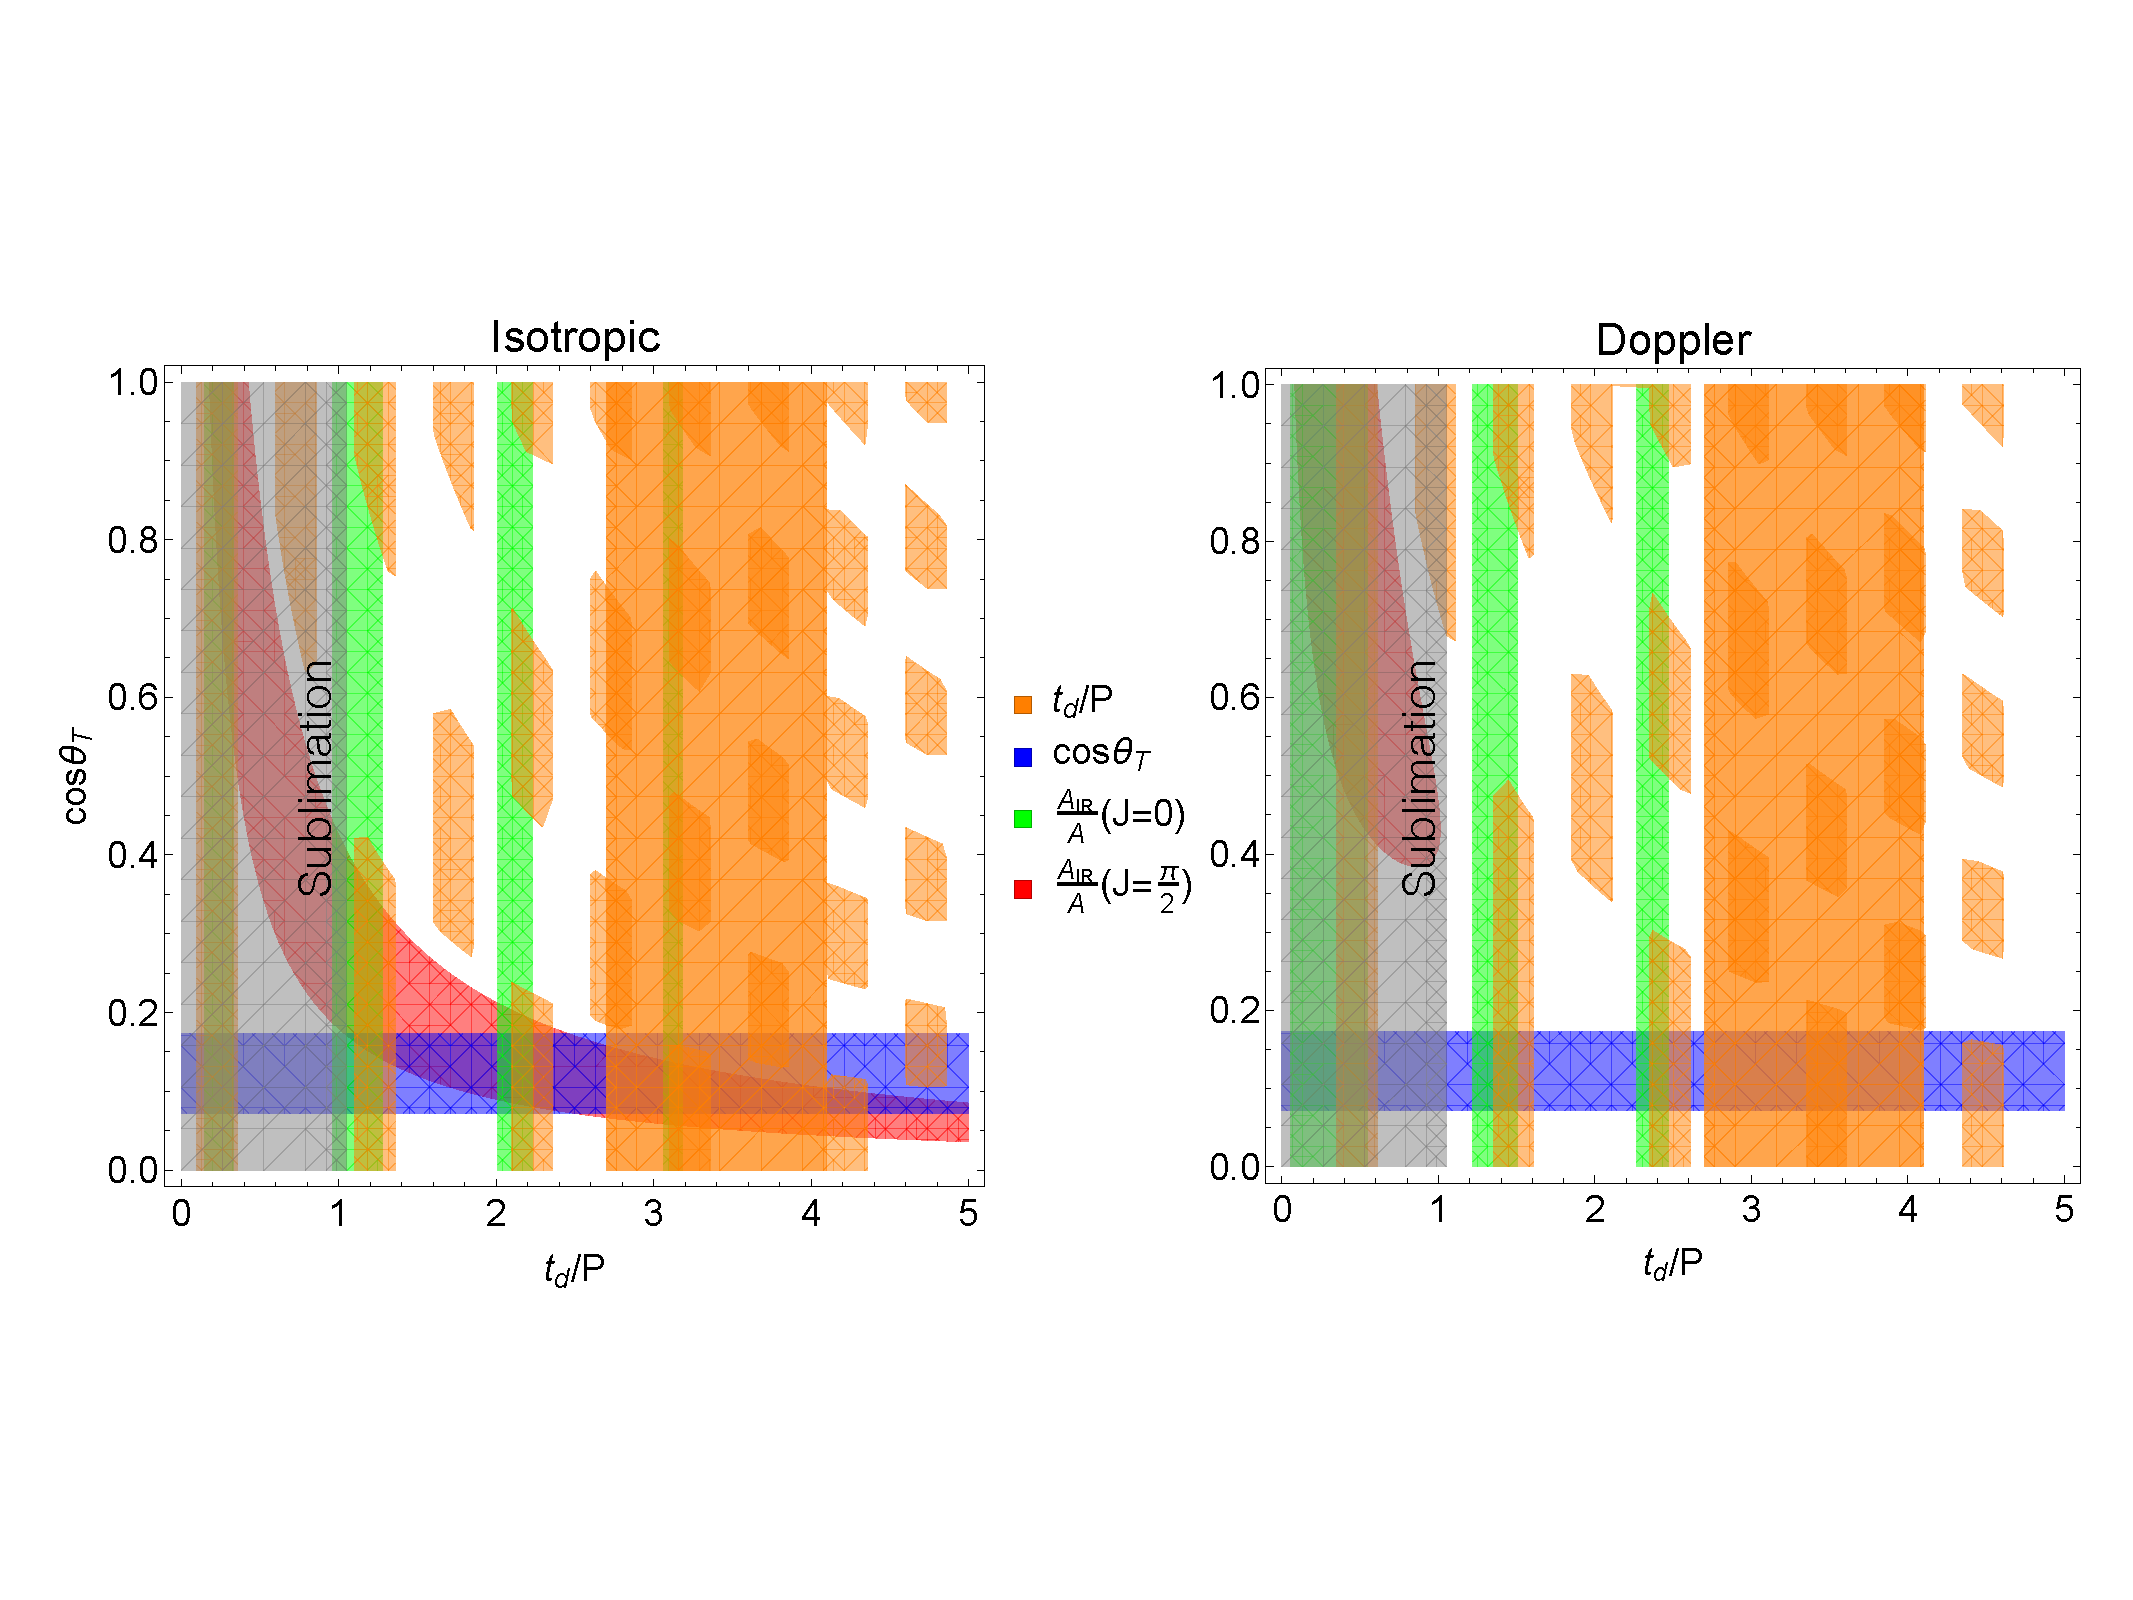
\includegraphics[scale=0.4]{figures/ch5/ParamConts_Iso_Dop} \\ 
% 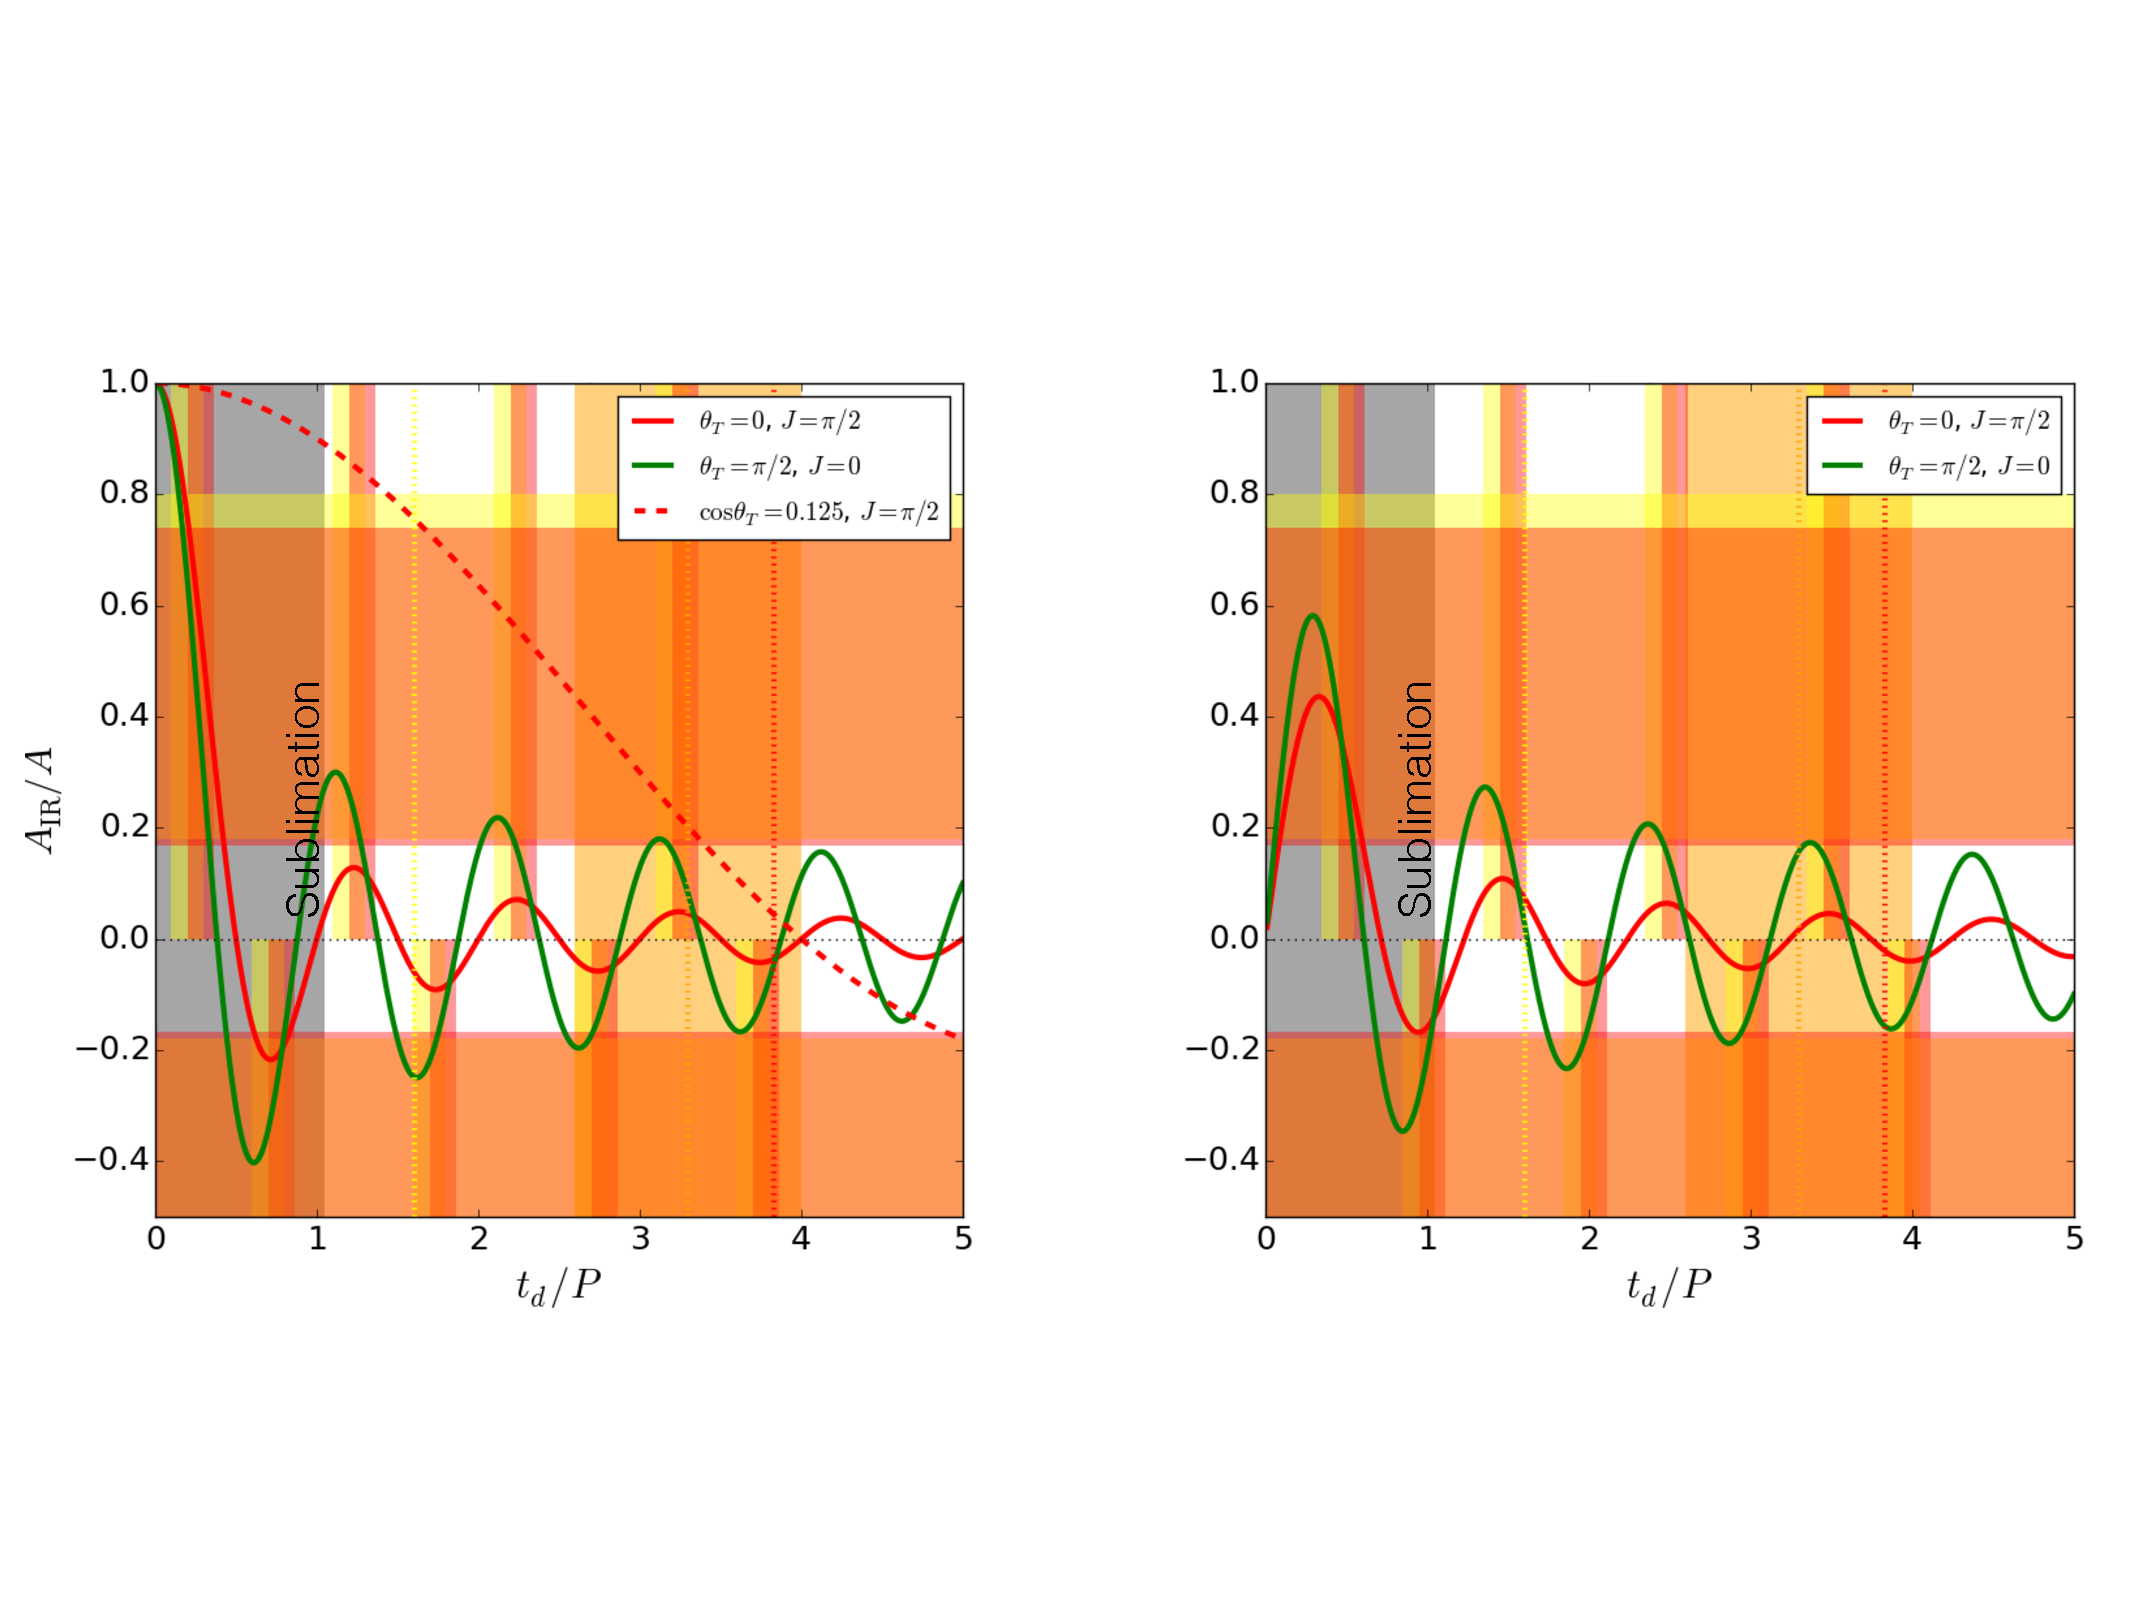
\includegraphics[scale=0.4]{figures/ch5/AIRA_tdoP_ParamSpace_Iso_Dop}
% \end{array}$
% \end{center}
% %
% \caption{
% Regions of allowed parameter space for torus models of dust surrounding a MBHB
% in PG 1302. See the text for details.}
% %
% \label{Fig:PGConts}
% \end{figure}



% %Fits
% \subsubsection{Light Curve fitting}

% Finally we calculate W1 and W2 IR light curves numerically, via the formulae
% laid out in \S \ref{S:Derivation}), and fit them to the WISE W1 and W2 data.
% For both isotropic and Doppler models we fit the radius of the dust shell
% $R_d$, the torus opening angle $\theta_T$, the torus inclination angle $J$,
% and the average magnitude of the W1 band light curve, mag$^{\rm{W1}}_0$. We
% vary mag$^{\rm{W1}}_0$ because in the previous section we found a discrepancy
% between the derived values of the dust sphere radius  which could have
% resulted from the assumption that the IR SED of PG 1302 is a pure black body
% being emitted by grains in a smooth density distribution. Because the SED is
% likely not a pure blackbody \citep[\textit{{e.g.}}][]{Netzer:2015:rev}, we
% escape this inconsistency by allowing the SED to vary, by allowing the average
% W1-band flux to vary. 

% \textcolor{red}{Testing now if solutions change when
% both W1 and W2 are allowed to vary}



% Figure \ref{Fig:PGBestFits} shows the best fit light curves for isotropic
% (left) and Doppler-boost (right) sources and Table \ref{Table:PGFit} displays
% the best fit parameters and their upper and lower $15^{\rm{th}}$ percentile
% errors.


% The best fit dust models are in accordance with the parameter constraints
% determined from analytical reasoning above. The best fit dust structure around
% the isotropic source is a nearly face on disc with a reduced chi-squared
% goodness of fit statistic $\chi^2_{\rm{red}} = 2.08$. The best fit dust
% structure around the Doppler-boosted source is a nearly edge on ring with
% $\chi^2_{\rm{red}} = 1.52$. Employing the Bayesian information criterion to
% compare the two models we find that $\rm{BIC} = 6.72$, strongly favoring the
% Doppler model.


% While the Doppler fit is favored, it poses two problems. The first and most
% serious is that an edge on disc which absorbs UV/optical light would obscure
% the central source, and PG 1302 is not a dust obscured Quasar. The largest
% possible torus inclination in the Doppler case is $\sim 1.5^{\circ}$ while the
% smallest angle that the dust could subtend is $\sim 6.6^{\circ}$. The second
% problem, though less serious, is that the best fit dust radius is outside of
% that predicted by the SED fitting above; this is apparent in the larger value
% of mag$^{\rm{W1}}_0$, and hence larger deviation from the best-fit blackbody
% SED, required by the Doppler model.



% Because of these issues with the best-fit Doppler model, we conclude that the
% case of an isotropically varying central source, surrounded by a nearly face-
% on dust disc is the only model consistent with the IR and UV/optical data.
% This conclusion is of course made within the assumptions of our model: that the
% dust is in a smooth torus configuration, optically thick to UV/optical and
% optically thin IR dust emission. We leave for future work the relaxation of
% these assumptions and their consequence for the nature of PG 1302 variability
% and its nuclear dust.


% %%%%%%%%%%%%%%%%%%%%%%%%%%%%%%%%%%%%%%%%%%%%%%%%
% %%% FIGURE: Sphere IR light curves ISO vs Dop%%%
% %%%%%%%%%%%%%%%%%%%%%%%%%%%%%%%%%%%%%%%%%%%%%%%%
% \begin{figure}
% \begin{center}$
% \begin{array}{c c}
% %FISO and DOP  vary Rin
% 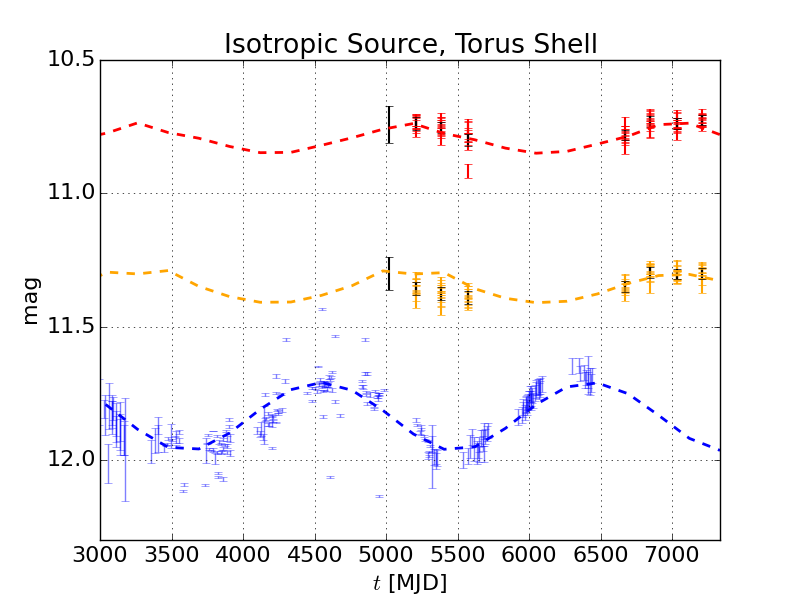
\includegraphics[scale=0.36]{figures/ch5/FinalFits/Test_ISO_mag0s_noRpriors_GeoThin_OptThin_noAMP_Tsub1800BestFit.png} & 
% 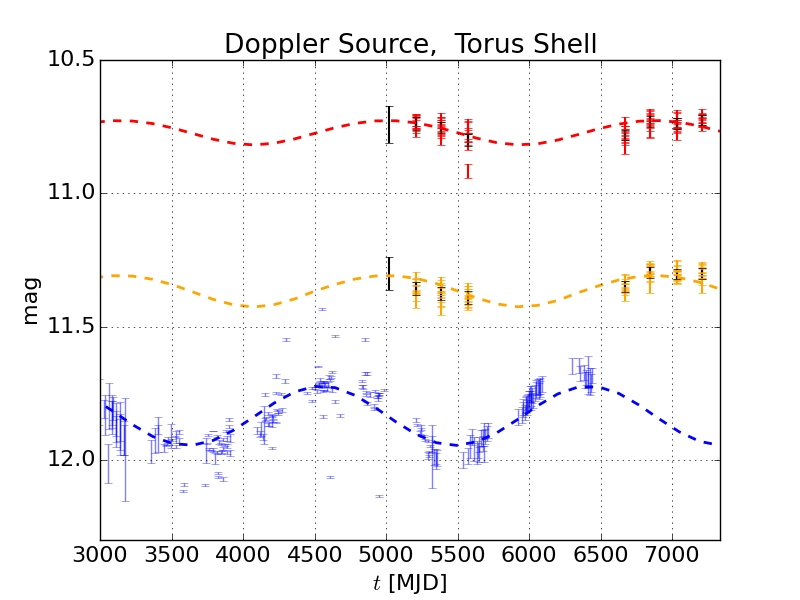
\includegraphics[scale=0.36]{figures/ch5/FinalFits/Test_DOP_GeoThin_OptThin_Fitmag0W1_NTemp1800_Tsub1800_BestFit}
% \end{array}$
% \end{center}
% %
% \caption{
% The best fit optical (blue), W1 (orange), and W2 (red) light curves for PG
% 1302 assuming an isotropically varying source (left) and a Doppler-boosted
% source (right). The WISE data is binned into six month epochs (black data
% points) by taking the average mean and standard deviation of the $\sim 10$
% data points at each six month epoch (orange and red data points).
% }
% %
% \label{Fig:PGBestFits}
% \end{figure}




% %DD explain reason for solutions - rings can get hi amps 


% %%%%%%%%%%%%%%%%%%%%%%%%%%%%%%%%%%%%%%%%%%%%%%%%



% \begin{table}
% \begin{center}
% \begin{tabular}{ c | c | c }
% %
%                      &      Isotropic              &  Doppler                    \\
% \hline
% $R_d$ [pc]           &  $2.91^{+0.05}_{-0.05}$     &  $1.224^{+0.005}_{-0.006}$  \\ \\
% $\cos{\theta_T}$     &  $0.124^{+0.002}_{-0.003}$  &  $0.117^{+0.012}_{-0.003}$  \\ \\
% $\sin{J}$            &  $0.991^{+0.001}_{-0.003}$  &  $0.012^{+0.014}_{-0.003}$  \\ \\
% mag$^{\rm{W1}}_0$    &  $0.016^{+0.011}_{-0.001}$  &  $0.537^{+0.005}_{-0.002}$  \\ 
% \hline      
% $\chi^2_{\rm{red}}$  &  $1.52$                     &  $2.08$ 
% %
%  \end{tabular}
% \caption{
% The best fit parameters for fits to the WISE W1-band and W2-band data assuming
% isotropic and Doppler boosted sources. We have used a simple reduced chi-
% squared $\chi^2_{\rm{red}}$ goodness of fit statistic to compare the two fits,
% the Doppler source model fits marginally better than the isotropic model.
% }
%  \end{center}
%  \label{Table:PGFit}
% \end{table}












































































\section{Discussion}
\label{S:Discussion}
We summarize our key results and discuss their implications for MBHBs.

\begin{enumerate}
%
\item{ 

\textbf{The phase lag of IR variability} relative to UV/optical variability is
given by $2 \pi t_d/P$ radians in the isotropic case and $2 \pi t_d/P(1 +
1/4)$ radians in the Doppler case. This important difference, for periodic
sources, should be considered when simply relating an IR time lag with the
light travel time across the dust reverberation region.

We also point out that there is an additional half-cycle phase shift for light
curves which are reflection symmetric (sinusoids). Whether this phase
shift occurs depends on the value of $t_d/P$ (see Eq. (\ref{Eq:LIR_thT})) and is
important for determining the size of the emitting dust region through IR
phase lags. 

}

\item{   

\textbf{The amplitude of IR variability} relative to UV/optical  is a function
of the ratio of dust light crossing time to variability period $t_d/P$, the
inclination and opening angles of the dust torus, and also the binary
inclination to the line of sight for a Doppler-boosted source (see Figures
\ref{Fig:AIRoAUV_tr} and \ref{Fig:AIRoAUVDop_tr}). In the isotropic case, the IR amplitude falls to zero for
$t_d/P \gg 1$, and approaches that of the UV/optical continuum for $t_d/P
\rightarrow 0$.  The Doppler case obtains peak amplitude at $t_d/P \sim 0.3
\rightarrow 0.6$, depending on the torus properties, and falls to zero for
both $t_d/P \rightarrow 0$ and $t_d/P \gg 1$. The isotropic case exhibits zero
relative IR amplitude at $t_d/P \cos{\theta_T} = m/2$ while the Doppler case
exhibits zero relative IR amplitude at $t_d/P \cos{\theta_T} + 1/4 \approx
m/2$.


Using Eq. (\ref{Eq:Rd}), we relate the value of $t_d/P$ to the mass of the
binary (through the Eddington limit) and the variability period,
\begin{equation}
t_d/P \gsim 0.7 \left(\frac{P}{4 \rm{yr} } \right)^{-1} \left(\frac{M}{10^9 \Msun } \right)^{1/2}.
\end{equation}
which provides a lower limit because we have identified $t_d$ with the dust sublimation radius.
Contours of $t_d/P$ are overlaid in Figure \ref{Fig:boostParams}. From Figure
\ref{Fig:boostParams} and Figure \ref{Fig:AIRoAUV_sp}, we conclude that, for
isotropic sources, long period and low mass binaries generate the largest
IR modulations. If the variations are due to the Doppler boost, however, low
mass binaries on long period orbits create weak UV/optical variations to start
with, and more intermediate masses and binary periods are favored for
detection of variability in the IR. 

}


\item{

\textbf{Orphan-IR variability} can occur for Doppler sources which are nearly
face-on (so we do not see the UV/optical variability), but are surrounded by a
dust torus which is not symmetric between the front and back of the Doppler
boost source. Such orphan-IR periodicity in quasars could be a smoking gun
signature of Doppler-boosted MBHBs at high binary inclination to the line of sight,
and would not as yet been identified in optical searches such as those carried
out by \cite{Graham+2015b} and \cite{Charisi+2016}. 

}

% \item{ 

% \textbf{Periodic IR variability from PG 1302} is consistent with reverberation
% of an isotropically varying source by a nearly face-on, dust-disc structure
% with aspect ratio $0.13 \pm 0.06$ and radius $R_d \sim 4.2 \pm 0.7$ pc. The
% best fit model to the IR data is for reverberation of a Doppler boosted source
% by a nearly edge-on disc with aspect ratio $0.13 \pm 0.06$ and radius $R_d
% \sim 1.7 \pm ??$ pc. However, all the dust models in this work assume that the
% dust is optically thick to UV/optical radiation and this best-fit Doppler model
% would be obscured by an edge-on dusty ring. We conclude that the
% isotropically varying scenario is the most compelling within the limitation of
% our dust modeling, but future work should extend these models to determine the
% feasibility of the Doppler-boost scenario.

% }


\end{enumerate}


 


We list caveats and possible extensions to this work: 
\begin{itemize}

\item{ 

We have considered smooth, single species dust models which are optically thin
to their own emission and optically thick to UV/optical emission. Future work
should consider dust models which include dust heating by UV/optical over a
finite radial extent, IR absorption by dust, clumpy dust
\citep[\textit{e.g}][and references therein]{Netzer:2015:rev}, and a
distribution of dust grain species and sizes. 

}



\item 
We have assumed that the relative location of the emitting secondary is small
compared to the dust torus inner radius. Because of finite light travel times,
the relative motion of the binary with respect to the dust torus becomes
important on the level of the ratio of the binary separation and the size of
the IR reprocessing region (the dust). The ratio of binary separation to
torus inner edge is
\begin{equation}
\frac{a}{R_d} \simeq 0.008\ \epsilon_{1} \left(\frac{M}{10^9 \Msun}\right)^{-1/6}  \left(\frac{P}{5 \rm{yr}}\right)^{2/3}  \left(\frac{T}{1800 \rm{K}}\right)^{2.8},
\label{Eq:aORd}
\end{equation}
telling us that the impact of binary orbital motion on the time lags of
reprocessed light is most important for the lowest mass binaries with the
longest periods, and contribute on at most the few percent level for the
fiducial values taken here for a PG1302-like binary. Because the dependence on
mass is weak, and 5 years is a current upper limit on observed binary periods
discovered in EM time-domain surveys \citep[\textit{e.g.}][]{Graham+2015b}, it
is safe to assume that the effect of binary orbital motion is a $\lsim 2\%$
effect.

It will be important to take this effect into account for modeling the effects
of Doppler-boosted emission on the closer-in broad line regions around MBHBs,
the subject of future work.


\item For Doppler-boosted sources, we assume the binary to be on a circular
orbit. Some hydrodynamical models of the binary interaction with a gas disc
predict the excitation of large binary eccentricities
\citep{Roedig:2011:eccevo}. Such binary eccentricities will change the shape
of the optical and hence the IR light curves predicted here.





 \item If grains can re-form on a timescale shorter than a binary orbital
time, the inner   sublimation radius will change periodically with the
changing central source flux. From Eq. (\ref{Eq:Rd}), the change in dust
sublimation due to the changing observed luminosity variations $\delta L$ is
 \begin{equation}
 \frac{\delta R_d}{R_d} = \frac{1}{2} \frac{\delta L}{L}.
 \end{equation}
For typical Doppler luminosity variations, this could result in changes to the
inner dust radius of a few to $\sim 10 \%$, with the largest variations
occurring for less massive binaries with shorter periods. The dust will emit at a
constant (source-frame) temperature, but light travel time lags will be time
dependent.


\item General relativistic time delays and precession could become important.% \citep[e.g.][]. 
%http://arxiv.org/abs/1604.02148


\end{itemize}


\section{Conclusions}
\label{S:conclusions}

We have developed a model to compute IR light curves that result from the
reverberation of a periodic optical/UV source by dust. We consider two types
of central continuum sources: isotropically emitting sources, and sources for
which the continuum periodicity is caused by the relativistic Doppler boost,
resulting in an anisotropically varying source which heats the dust in a
lighthouse-like fashion. The latter is presented here for the first time. We
assume that the dust is optically thick to UV/optical radiation and optically
thin to IR emission and is configured in a torus centered on the continuum
source. We show that the phase, amplitude, and average brightness of
reverberated IR radiation is dependent on the ratio of light travel time
across the emitting dust region to the period of variability, the torus
opening angle, and the inclination of the torus to the line of sight. In the
case of Doppler-boosted emission, the IR (and continuum) emission depends also
on the inclination of binary orbital plane and dust torus.



% We applied our models to the sub-pc MBHB candidate PG 1302
% \citep{Graham+2015a}. We find two combinations of dust torus and source models
% that are consistent with the UV, optical and IR data. Either the periodic
% UV/optical variability from PG 1302 is isotropic and the dust is in the
% configuration of a disc-like (torus opening angle of $\sim 83^{\circ}$), face-
% on dust torus with radius $R_d \sim 4.2$ pc, or the central source is
% exhibiting variability due to Doppler boosting and is surrounded by a nearly
% edge-on disc-like torus at a closer distance of $\sim 1.7$ pc. The latter
% model is ruled out because of an edge-on disc would obscure the UV/optical
% emission form PG 1302, which is not observed.  The possible models can be
% narrowed down in the future by obtaining better IR spectral energy
% distribution for PG 1302 and by continual monitoring of PG 1302's optical, UV,
% and IR continuum.


This model will not only be useful for interpreting the nature of existing
MBHB candidates, but could help to discover more. If the binary's orbit is
highly inclined to the line of sight, but not to the dust structure, then an
imprint of Doppler boosting will not appear in the optical and UV, but it will
appear in the IR. This motivates a search for such orphan-IR Doppler imprints.

Future work will expand these models to incorporate more sophisticated dust
structures and radiative transfer. These along with the models and intuition
developed here will be applied to fit the IR light curves of the growing list
of MBHB candidates \citep{Graham+2015b, Charisi+2016, Jun:2015}. This will aid
in the interpretation of such sources as MBHBs, and also illuminate their
surrounding, dusty environments.




\section*{Acknowledgments} 
The authors thank Hyunsung Jun for providing the WISE data from his analysis,
including the average W1, W2, W3, and W4 fluxes. The authors also thank Hyunsung
Jun, Daniel Stern, Arlin Crotts, Jules Halpbern, Andrew MacFadyen, Jeffery J.
Andrews, and Adrian Price-Whelan for useful
discussion. DJD would like to thank Janna Levin and Pioneer Works for
providing a stimulating working space during the completion of this work. We
acknowledge support from a National Science Foundation Graduate Research
Fellowship under Grant No. DGE1144155 (DJD) and NASA grant NNX11AE05G (ZH).










\renewcommand\thesection{\thechapter.\arabic{section}}